\chapter{Caso de estudio IMU y PID}
\label{ch:especifico3}

\section{Caso de estudio 2 - IMU}

Como caso de estudio de implementación se desarrolló también la simulación de una Unidad de medición inercial, IMU por sus siglas en Ingles, se siguió el uso del modelo que se presenta en \cite{mathworks2024imu}. Este ejemplo muestra cómo generar y fusionar datos de sensores IMU usando MATLAB Simulink. Permitiendo modelar con precisión el comportamiento de un acelerómetro, un giroscopio y un magnetómetro, además de poder fusionar sus salidas para calcular la orientación.

Una IMU es un grupo de sensores que incluye un acelerómetro para medir aceleración y un giroscopio para medir velocidad angular. Frecuentemente, también se incluye un magnetómetro para medir el campo magnético de la Tierra. Cada uno de estos tres sensores produce una medición de tres ejes, constituyendo una medición de 9 ejes en total. Ademas de esto un Sistema de Referencia de Actitud y Rumbo (AHRS, por sus siglas en inglés) toma las lecturas de sensores de 9 ejes y calcula la orientación del dispositivo. Esta orientación se da en relación con el marco NED, donde N es la dirección del Norte Magnético. El bloque AHRS en Simulink logra esto usando una estructura de filtro de Kalman indirecto \cite{mathworks2024imu}.

\newpage
\subsection{Implementación en MATLAB Simulink}

\begin{figure}[h!]
    \centering
    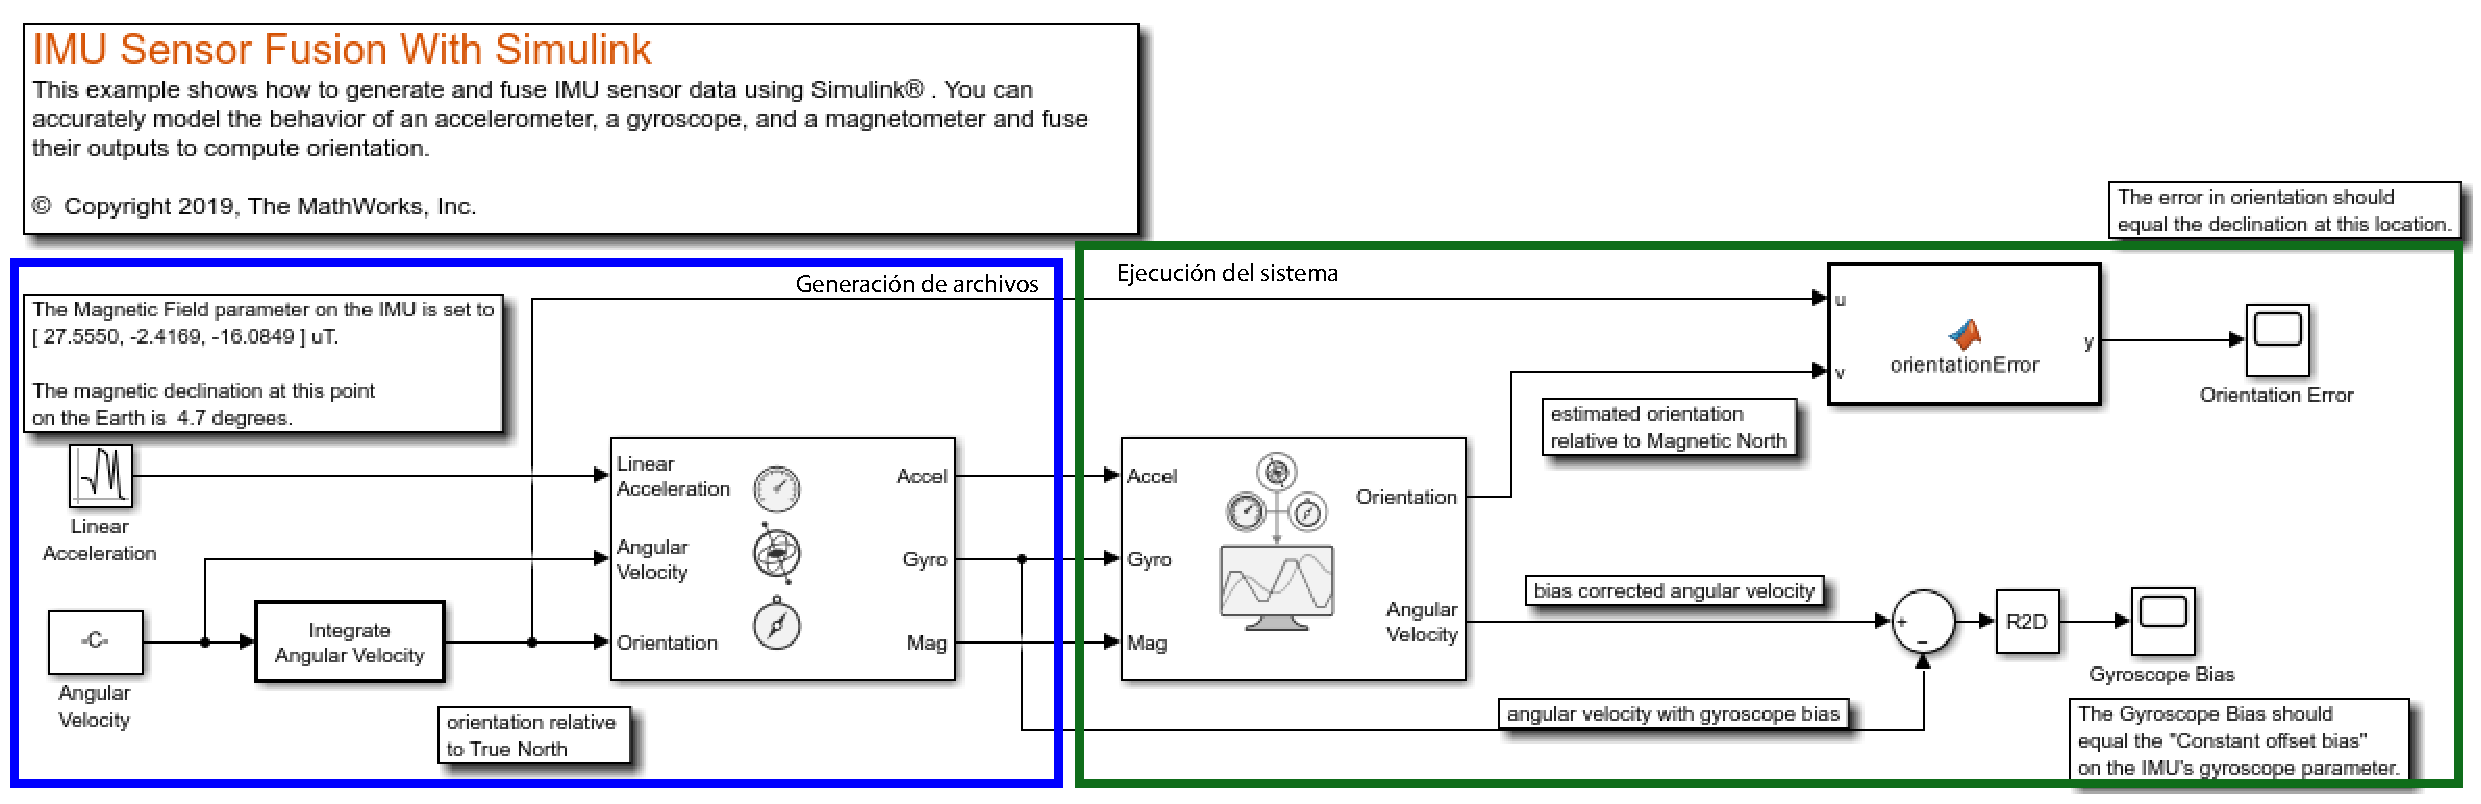
\includegraphics[width=0.8\textwidth]{fig/Capitulo5/Caso_de_estudio_IMU/FULL_IMU.pdf}
    \caption{Diagrama completo del caso de estudio 2 - IMU \cite{mathworks2024imu}}
    \label{fig:caso_de_estudio_2_IMU}
\end{figure}


Como se puede observar en la Figura \ref{fig:caso_de_estudio_2_IMU}, este es el caso de estudio que se propone en \cite{mathworks2024imu}, a este caso de estudio se le deben de realizar unas modificaciones de acuerdo al funcionamiento deseado que se tiene para este caso de estudio, siempre generando datos en el ámbito de simulación en MATLAB para luego contrastar los mismos con los datos obtenidos en la ejecución del modelo en la tarjeta de desarrollo seleccionada.

\subsection{Bloques utilizados para la implementación}

Los bloques utilizados se obtienen en la librería de bloques de MATLAB Simulink. A continuación se muestran los bloques requeridos, asi como la configuración de los mismos para la correcta operación del modelo. La implementación del sistema se divide en dos partes, el primer parte se encarga de generar los archivos necesarios para la operación del sistema mientras que la segunda parte del sistema se encarga de leer los archivos con los datos y generar los dos archivos de salida del programa.

\subsubsection{Sistema para la generación de archivos}\label{subsub:generación_de_archivos}

\begin{figure}[h!]
    \centering
    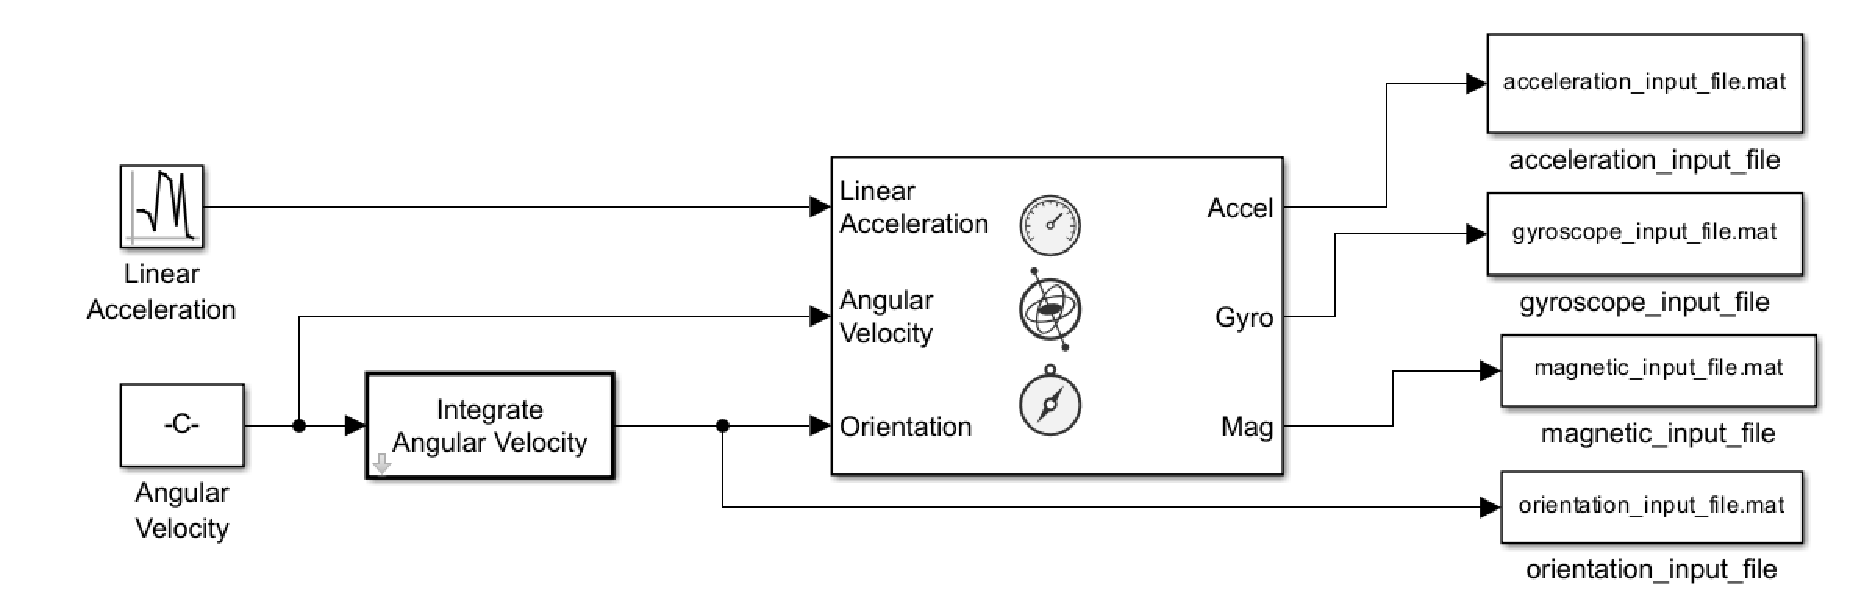
\includegraphics[width=0.8\textwidth]{fig/Capitulo5/Caso_de_estudio_IMU/Generador_de_archivos/flujo_generador_de_archivos.pdf}
    \caption{Diagrama utilizado para la generación de los archivos \cite{mathworks2024imu}}
    \label{fig:caso_de_estudio_2_IMU_generación_de_archivos}
\end{figure}

Este sistema es el encargado de generar los archivos de entrada, estos mismos contienen los datos de tiempo y valores para la correcta implementación del sistema, estos bloques se utilizarán para construir el diagrama de la Figura \ref{fig:caso_de_estudio_2_IMU_generación_de_archivos}.

\begin{figure}[htbp]
    \centering
    \begin{subfigure}[b]{0.45\textwidth}
        \centering
        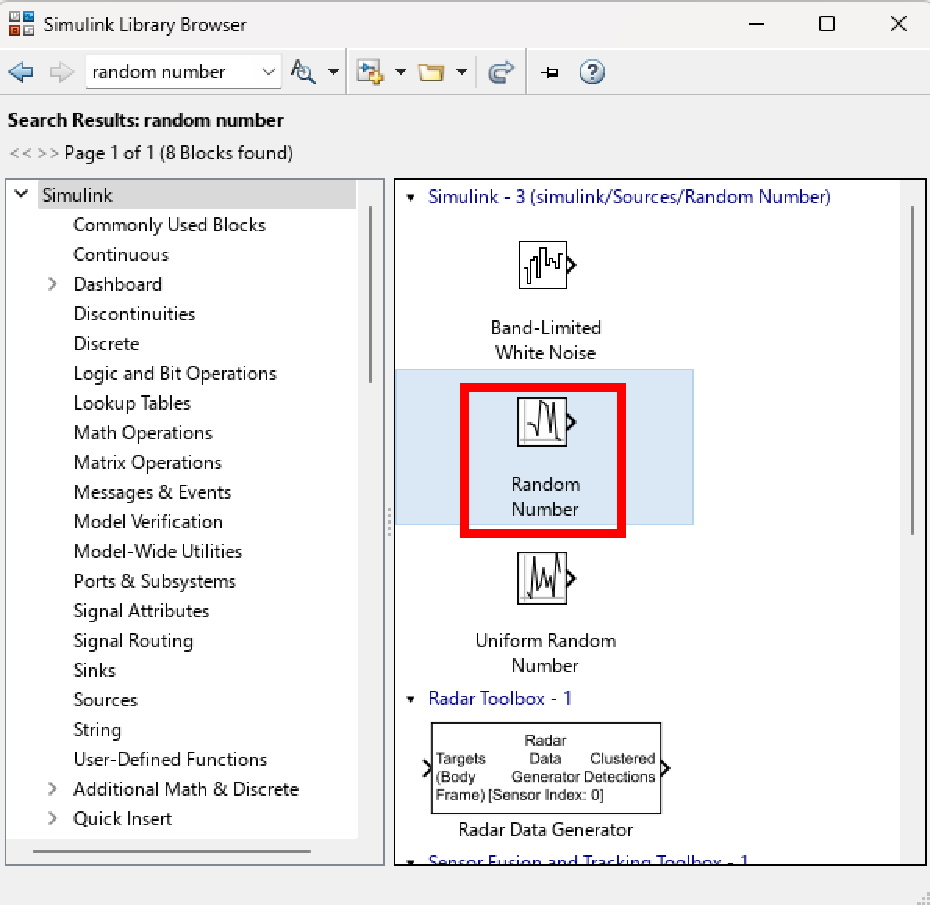
\includegraphics[width=\textwidth]{fig/Capitulo5/Caso_de_estudio_IMU/Generador_de_archivos/libreria_de_bloques_aceleracion_lineal.pdf}
        \caption{Librería de bloques - Aceleración Lineal}
        \label{fig:lib_bloques_linear_acceleration}
    \end{subfigure}
    \hfill
    \begin{subfigure}[b]{0.45\textwidth}
        \centering
        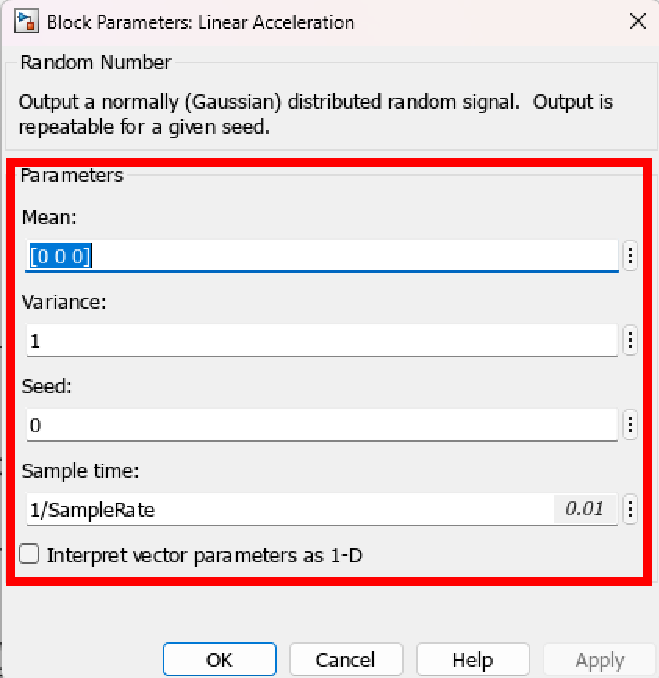
\includegraphics[width=\textwidth]{fig/Capitulo5/Caso_de_estudio_IMU/Generador_de_archivos/configuracion_bloque_aceleracion_lineal.pdf}
        \caption{Configuración del bloque aceleración lineal}
        \label{fig:lib_bloques_config_linear_acceleration}
    \end{subfigure}
    \caption{Bloque para la aceleración lineal}
    \label{fig:linear_accel_block_simulink}
\end{figure}

Como se pudo observar en la Figura \ref{fig:linear_accel_block_simulink}, se presenta a la izquierda la librería donde se encuentra el bloque a utilizar para establecer la constante de la velocidad angular, para este caso se utiliza en el mismo un valor de xxx, el mismo se observa en la Figura \ref{fig:lib_bloques_config_linear_acceleration}, además de algunas configuraciónes adicionales requeridas por el bloque. 

\begin{figure}[htbp]
    \centering
    \begin{subfigure}[b]{0.45\textwidth}
        \centering
        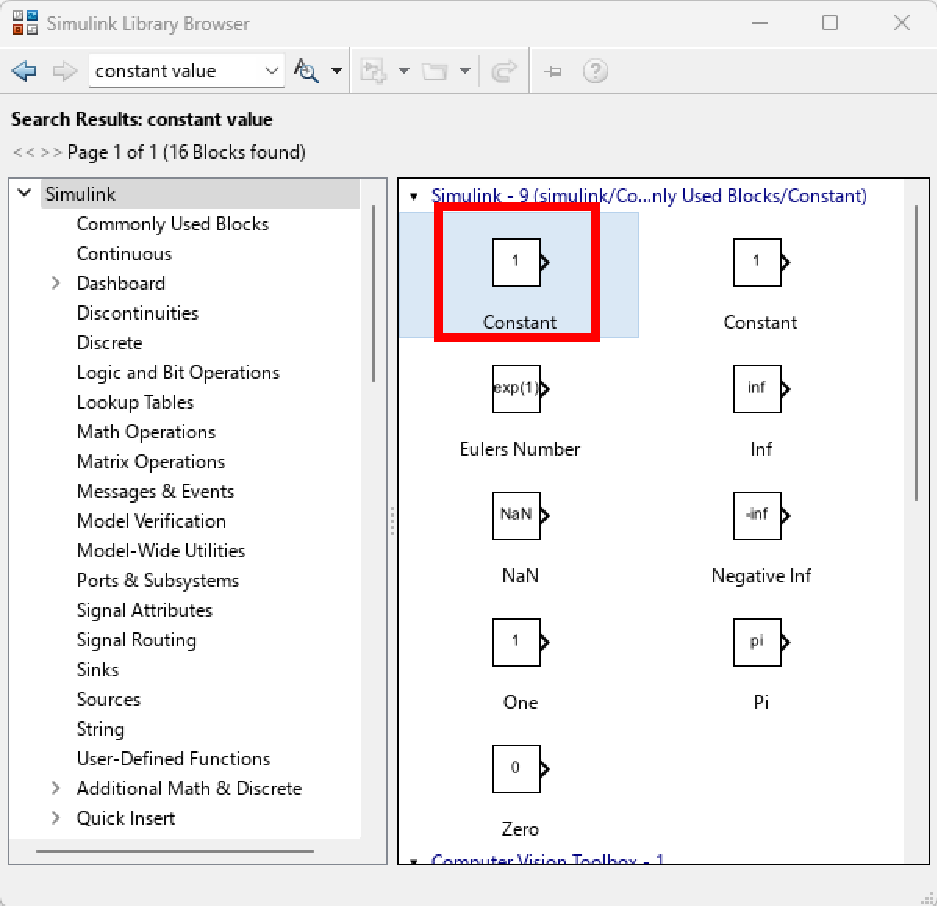
\includegraphics[width=\textwidth]{fig/Capitulo5/Caso_de_estudio_IMU/Generador_de_archivos/libreria_de_bloques_constante_velocidad_angular.pdf}
        \caption{Librería de bloques - Velocidad Angular}
        \label{fig:lib_bloques_angular_velocity}
    \end{subfigure}
    \hfill
    \begin{subfigure}[b]{0.45\textwidth}
        \centering
        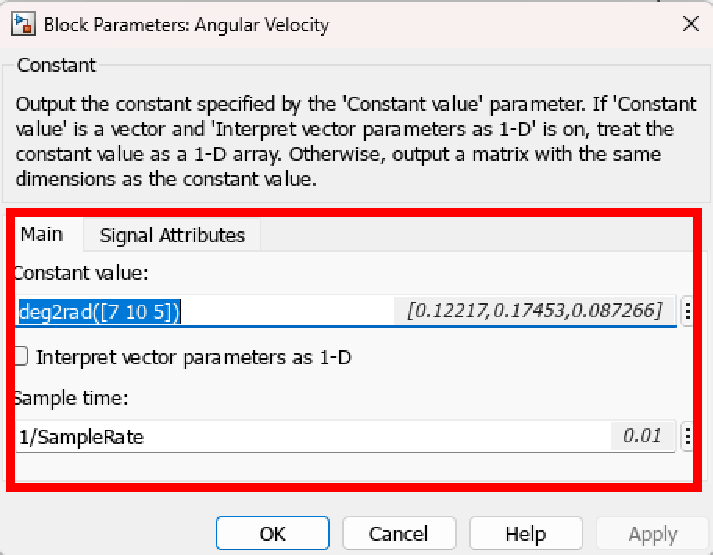
\includegraphics[width=\textwidth]{fig/Capitulo5/Caso_de_estudio_IMU/Generador_de_archivos/configuracion_bloque_velocidad_angular.pdf}
        \caption{Configuración del bloque velocidad angular}
        \label{fig:lib_bloques_config_angular_velocity}
    \end{subfigure}
    \caption{Bloque para la velocidad angular}
    \label{fig:angular_velocity_block_simulink}
\end{figure}

Seguido de esto, podemos observar en la Figura \ref{fig:angular_velocity_block_simulink} el bloque encargado de establecer la variable de la velocidad angular, a la izquierda se observa el bloque a utilizar en la librería y a la derecha se encuentra la configuración utilizada para este bloque. 

\newpage

\begin{figure}[htbp]
    \centering
    \begin{subfigure}[b]{0.35\textwidth}
        \centering
        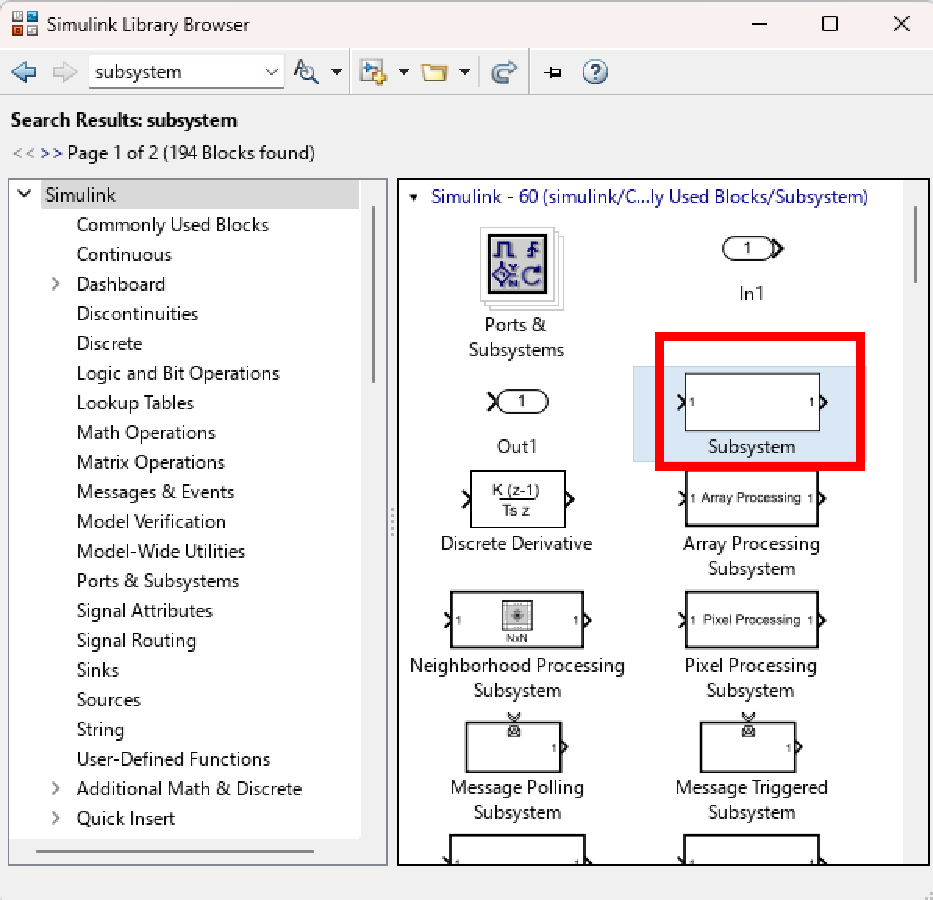
\includegraphics[width=\textwidth]{fig/Capitulo5/Caso_de_estudio_IMU/Generador_de_archivos/libreria_de_bloques_subsistema_integracion_velocidad_angular.pdf}
        \caption{Librería de bloques - Integrador}
        \label{fig:lib_bloques_integrador}
    \end{subfigure}
    \hfill
    \begin{subfigure}[b]{0.45\textwidth}
        \centering
        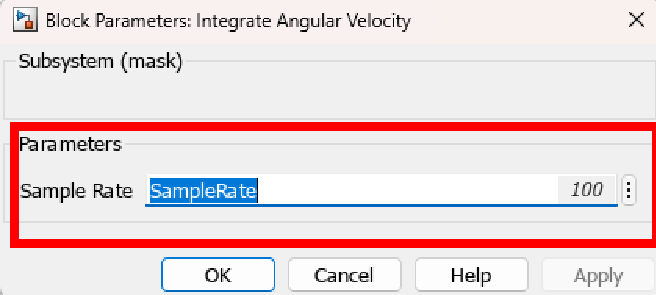
\includegraphics[width=\textwidth]{fig/Capitulo5/Caso_de_estudio_IMU/Generador_de_archivos/configuracion_integrador_velocidad_angular.pdf}
        \caption{Configuración del bloque velocidad angular}
        \label{fig:config_bloques_integrador}
    \end{subfigure}
    \caption{Bloque para la integración de la velocidad angular}
    \label{fig:integration_for_angular_velocity}
\end{figure}

Adicional al bloque que se observo en \ref{fig:angular_velocity_block_simulink} tambien se debe de implementar un bloque encargado de integrar el valor de la velocidad angular, para esto se usa el bloque que se muestra en \ref{fig:integration_for_angular_velocity}, este mismo lo podemos encontrar en la libreria de bloques de Simulink como se muestra en \ref{fig:lib_bloques_integrador}, tambien, en la Figura \ref{fig:config_bloques_integrador} se muestra la configuración utilizada en el bloque.
\newpage

\begin{figure}[htbp]
    \centering
    % Primera imagen
    \begin{subfigure}[b]{0.35\textwidth}
        \centering
        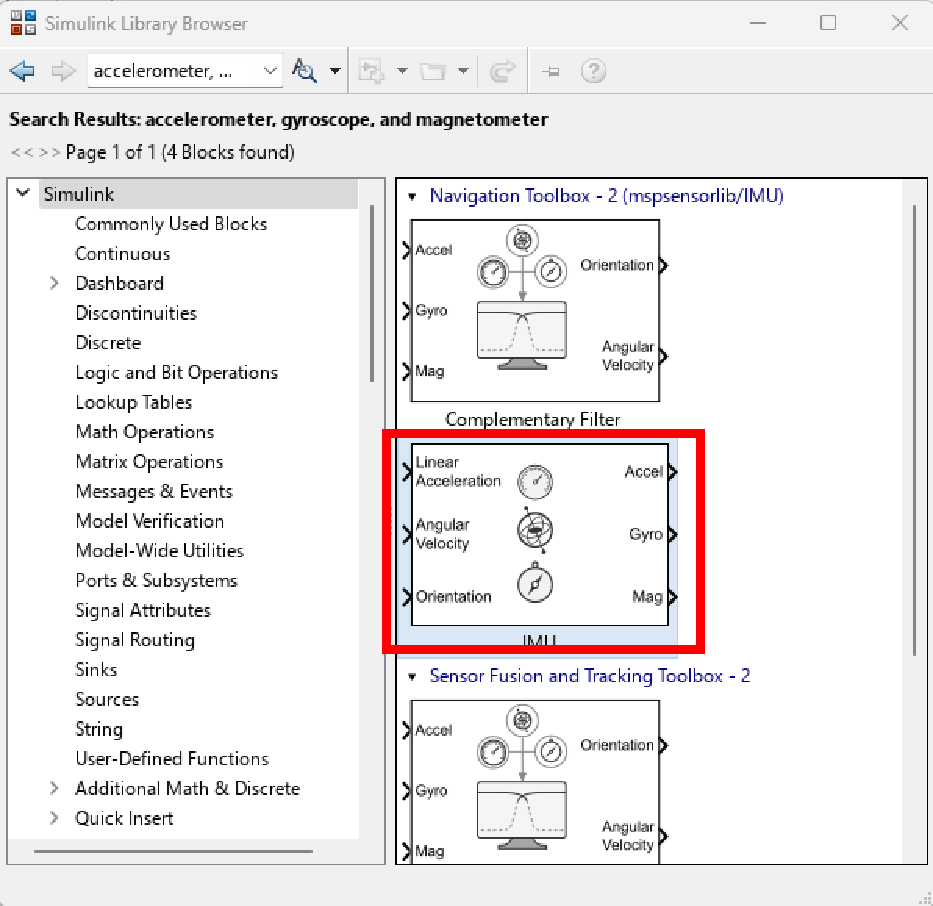
\includegraphics[width=\textwidth]{fig/Capitulo5/Caso_de_estudio_IMU/Generador_de_archivos/libreria_de_bloques_IMU.pdf}
        \caption{Librería de bloques - IMU}
        \label{fig:lib_bloques_IMU}
    \end{subfigure}
    \hfill
    % Segunda imagen
    \begin{subfigure}[b]{0.35\textwidth}
        \centering
        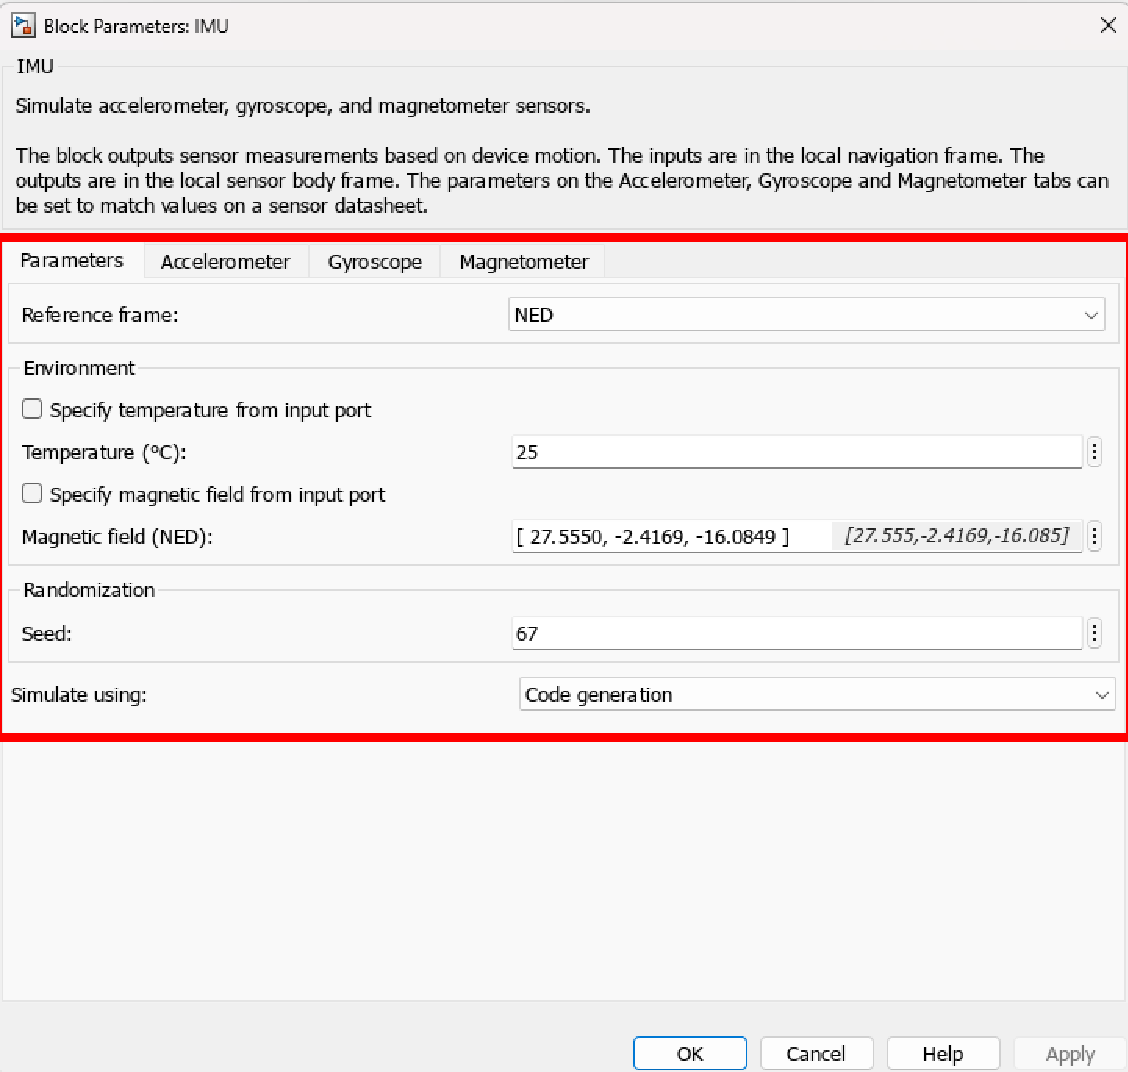
\includegraphics[width=\textwidth]{fig/Capitulo5/Caso_de_estudio_IMU/Generador_de_archivos/configuracion_parametros_IMU_01.pdf}
        \caption{Configuración de parámetros 1}
        \label{fig:parametros_IMU_01}
    \end{subfigure}
    \hfill
    % Tercera imagen
    \begin{subfigure}[b]{0.35\textwidth}
        \centering
        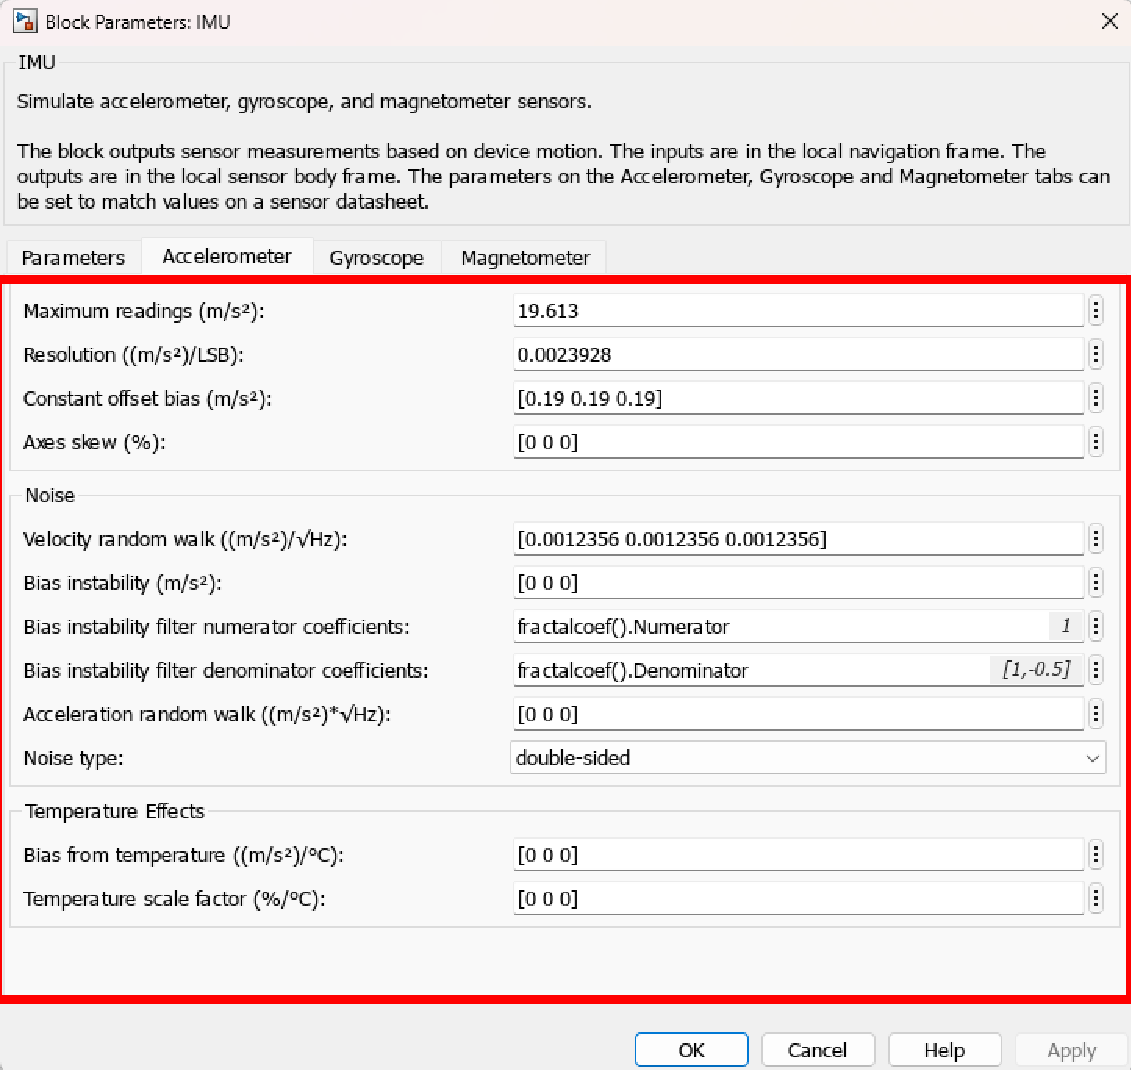
\includegraphics[width=\textwidth]{fig/Capitulo5/Caso_de_estudio_IMU/Generador_de_archivos/configuracion_parametros_IMU_02.pdf}
        \caption{Configuración de parámetros 2}
        \label{fig:parametros_IMU_02}
    \end{subfigure}
    \hfill
    % Cuarta imagen
    \begin{subfigure}[b]{0.35\textwidth}
        \centering
        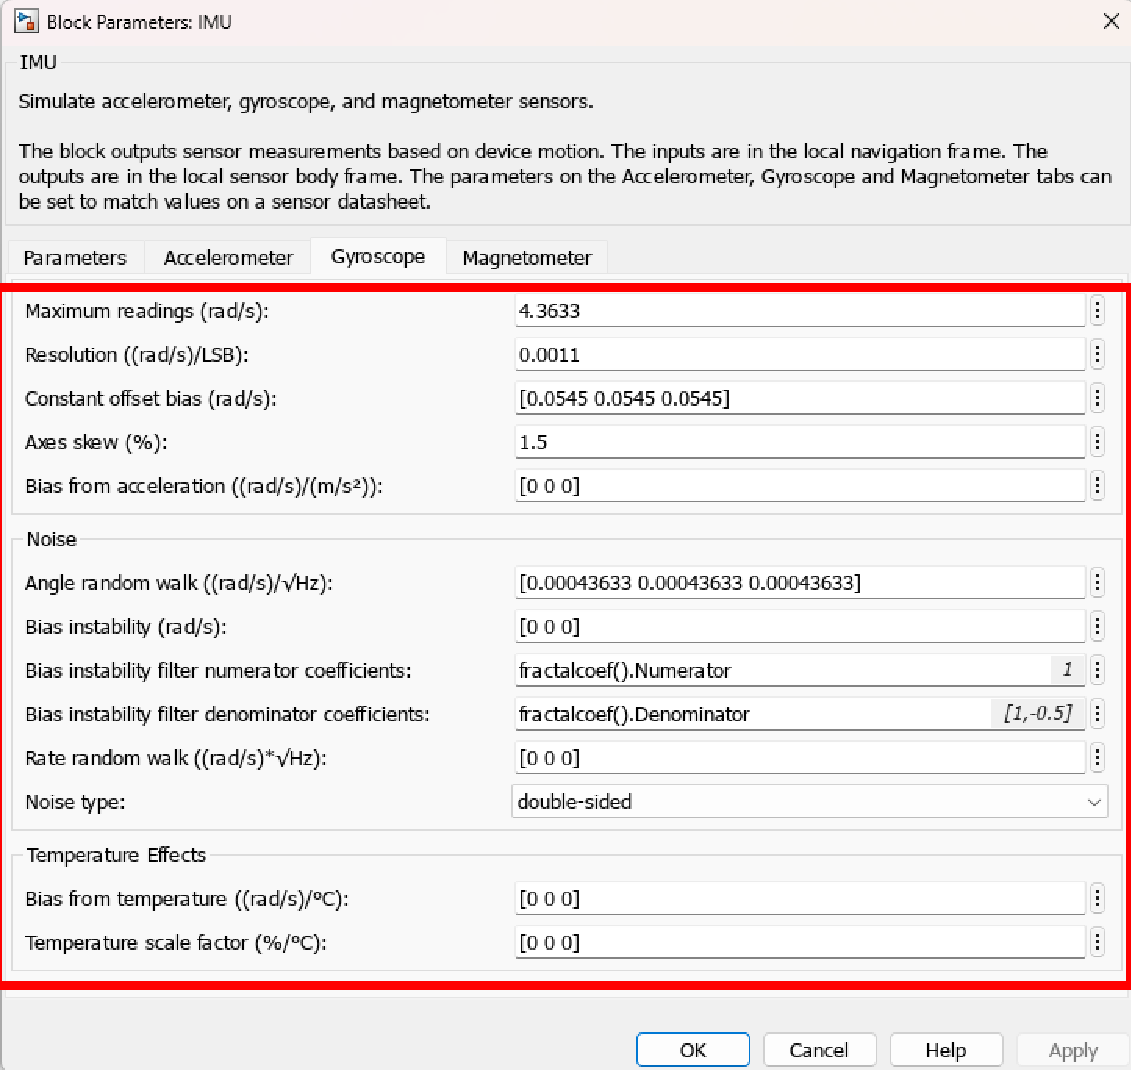
\includegraphics[width=\textwidth]{fig/Capitulo5/Caso_de_estudio_IMU/Generador_de_archivos/configuracion_parametros_IMU_03.pdf}
        \caption{Configuración de parámetros 3}
        \label{fig:parametros_IMU_03}
    \end{subfigure}
    \hfill
    % Quinta imagen
    \begin{subfigure}[b]{0.35\textwidth}
        \centering
        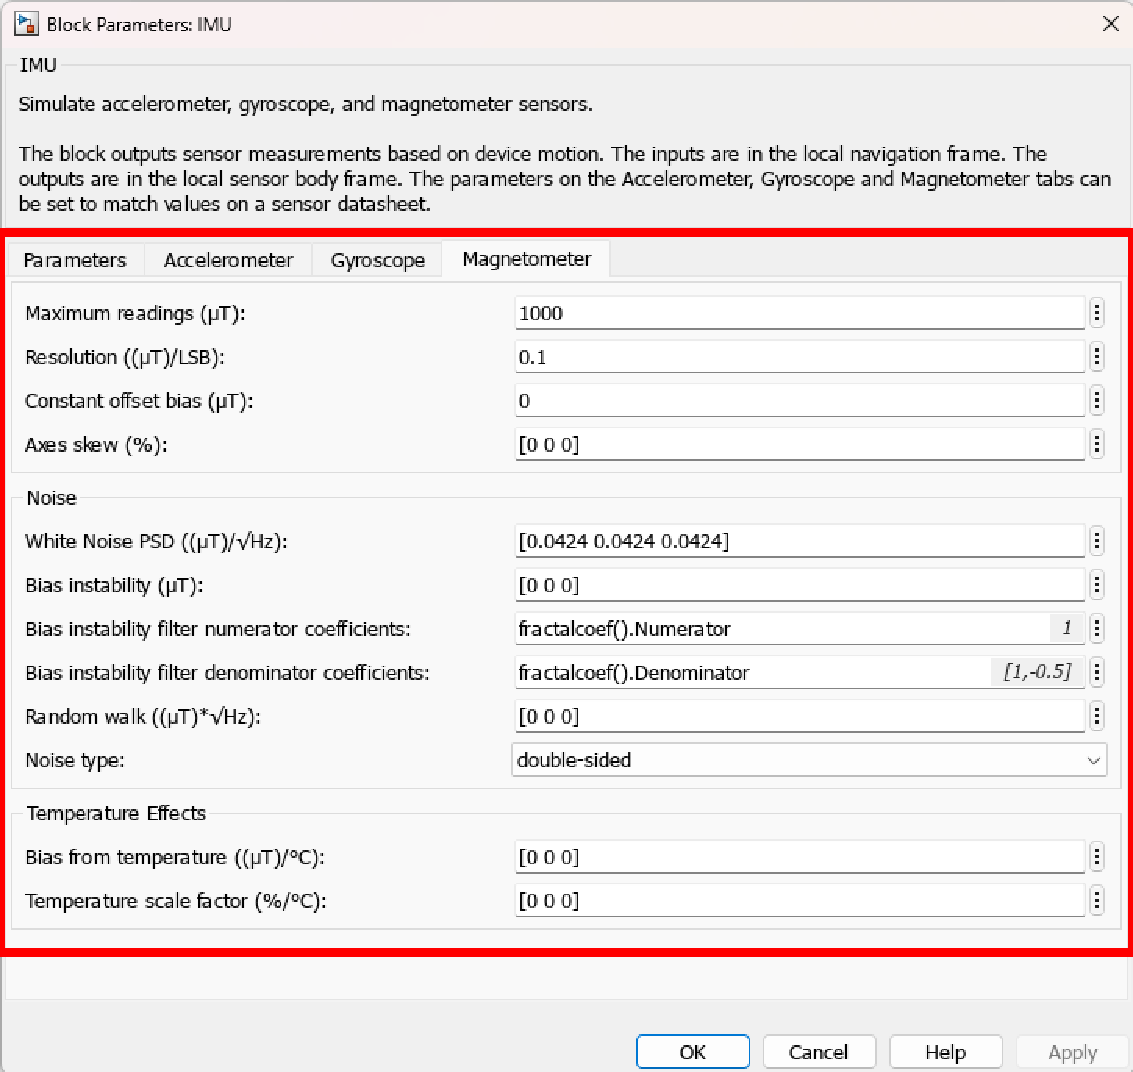
\includegraphics[width=\textwidth]{fig/Capitulo5/Caso_de_estudio_IMU/Generador_de_archivos/configuracion_parametros_IMU_04.pdf}
        \caption{Configuración de parámetros 4}
        \label{fig:parametros_IMU_04}
    \end{subfigure}

    \caption{Bloque para la simulación del comportamiento de la IMU}
    \label{fig:arreglo_imu}
\end{figure}


Finalmente en la Figura \ref{fig:arreglo_imu} se presenta el bloque encargado de simular la detección y medición de la aceleración y rotación en diferentes ejes de un sistema. Por un lado en la Figura \ref{fig:lib_bloques_IMU} se muestra el bloque en la librería. Por otro lado, en la Figura \ref{fig:parametros_IMU_01} se presenta la configuración del bloque respecto a los parámetros del mismo, esto contempla desde el marco de referencia a utilizar, la temperatura de operación del sistema, las componentes del campo magnético y la semilla, en la Figura \ref{fig:parametros_IMU_02} se presenta la configuración utilizada en el bloque para las componentes relacionadas con el acelerómetro, como se puede observar las mismas contemplan desde la configuración de máximos de lectura, resolución del sensor, el ruido y los efectos de temperatura, en la Figura \ref{fig:parametros_IMU_03} se presenta la configuración del boque relacionada a los parámetros del giroscopio, estos contemplan algunos parámetros similares a los del acelerometro y finalmente en la Figura \ref{fig:parametros_IMU_04} se muestra la configuración empleada para el magnetómetro. Cabe destacar que si se quiere replicar el experimento se deben de usar los parámetros mostrados en las imágenes contenidas en \ref{fig:arreglo_imu}. 




\begin{figure}[htbp]
    \centering
    \begin{subfigure}[b]{0.35\textwidth}
        \centering
        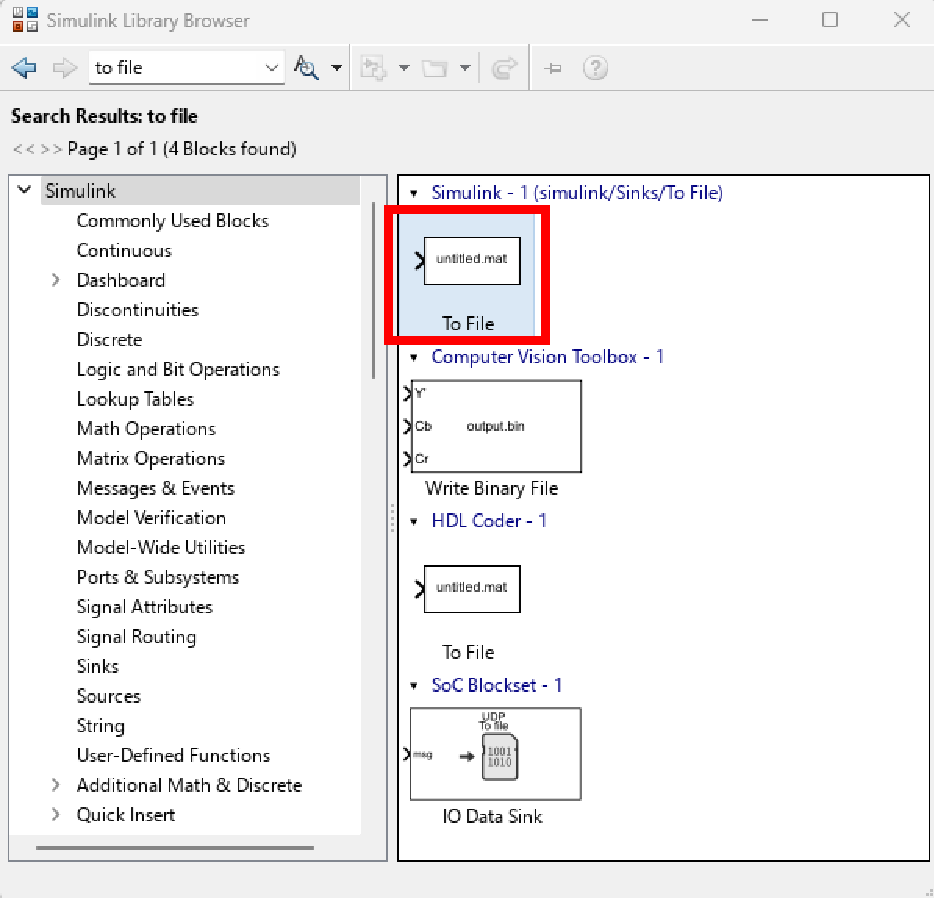
\includegraphics[width=\textwidth]{fig/Capitulo5/Caso_de_estudio_IMU/Generador_de_archivos/libreria_de_bloques_to_file.pdf}
        \caption{Librería de bloques - Guardar en archivo}
        \label{fig:lib_bloques_to_file_IMU}
    \end{subfigure}
    \hfill
    \begin{subfigure}[b]{0.45\textwidth}
        \centering
        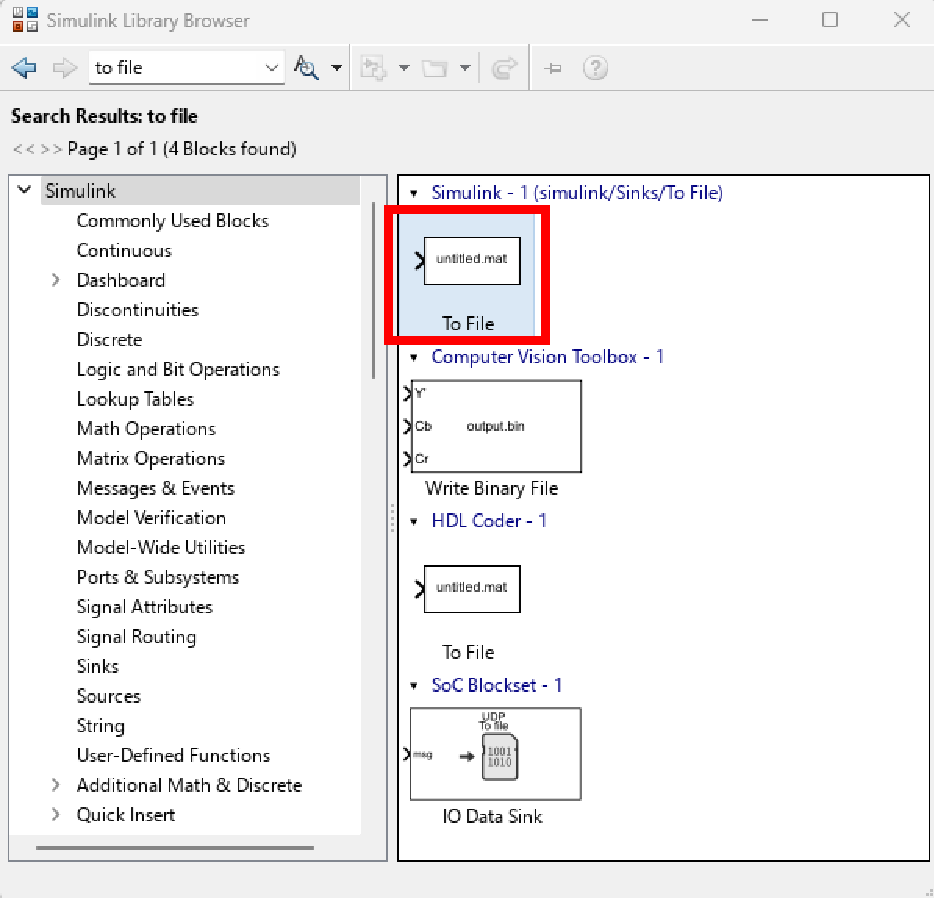
\includegraphics[width=\textwidth]{fig/Capitulo5/Caso_de_estudio_IMU/Generador_de_archivos/libreria_de_bloques_to_file.pdf}
        \caption{Configuración de parámetros - Guardar en archivo}
        \label{fig:config_to_file_IMU}
    \end{subfigure}
    \caption{Bloque para guardar los datos en un archivo}
    \label{fig:to_file_IMU}
\end{figure}

Para poder generar archivos los cuales se utilizaran más adelante en este flujo se utiliza el bloque que se muestra en la Figura \ref{fig:to_file_IMU}, este se encarga de generar un archivo en formato (.mat) con el objetivo de proveer datos a las otras secciónes de esta caso de estudio, cabe destacar que la configuración del mismo se muestra en la Figura \ref{fig:config_to_file_IMU} en donde se establece el nombre del archivo de salida, la forma de almacenamiento de los datos y finalmente el nombre de la variable por la cual se accederán estos datos. Los nombres a utilizar son:

\begin{itemize}
    \item acceleration\_input\_file
    \item gyroscope\_input\_file
    \item magnetic\_input\_file
    \item orientation\_input\_file
\end{itemize}

Estos nombres se deben de respetar a la hora de generar los archivos de salida, ya que el programa encargado de recibir estos datos buscara los archivos en el directorio bajo estos nombres.

\newpage

\subsubsection{Sistema para la lectura e interpretación de los archivos generados previamente}

\begin{figure}[h!]
    \centering
    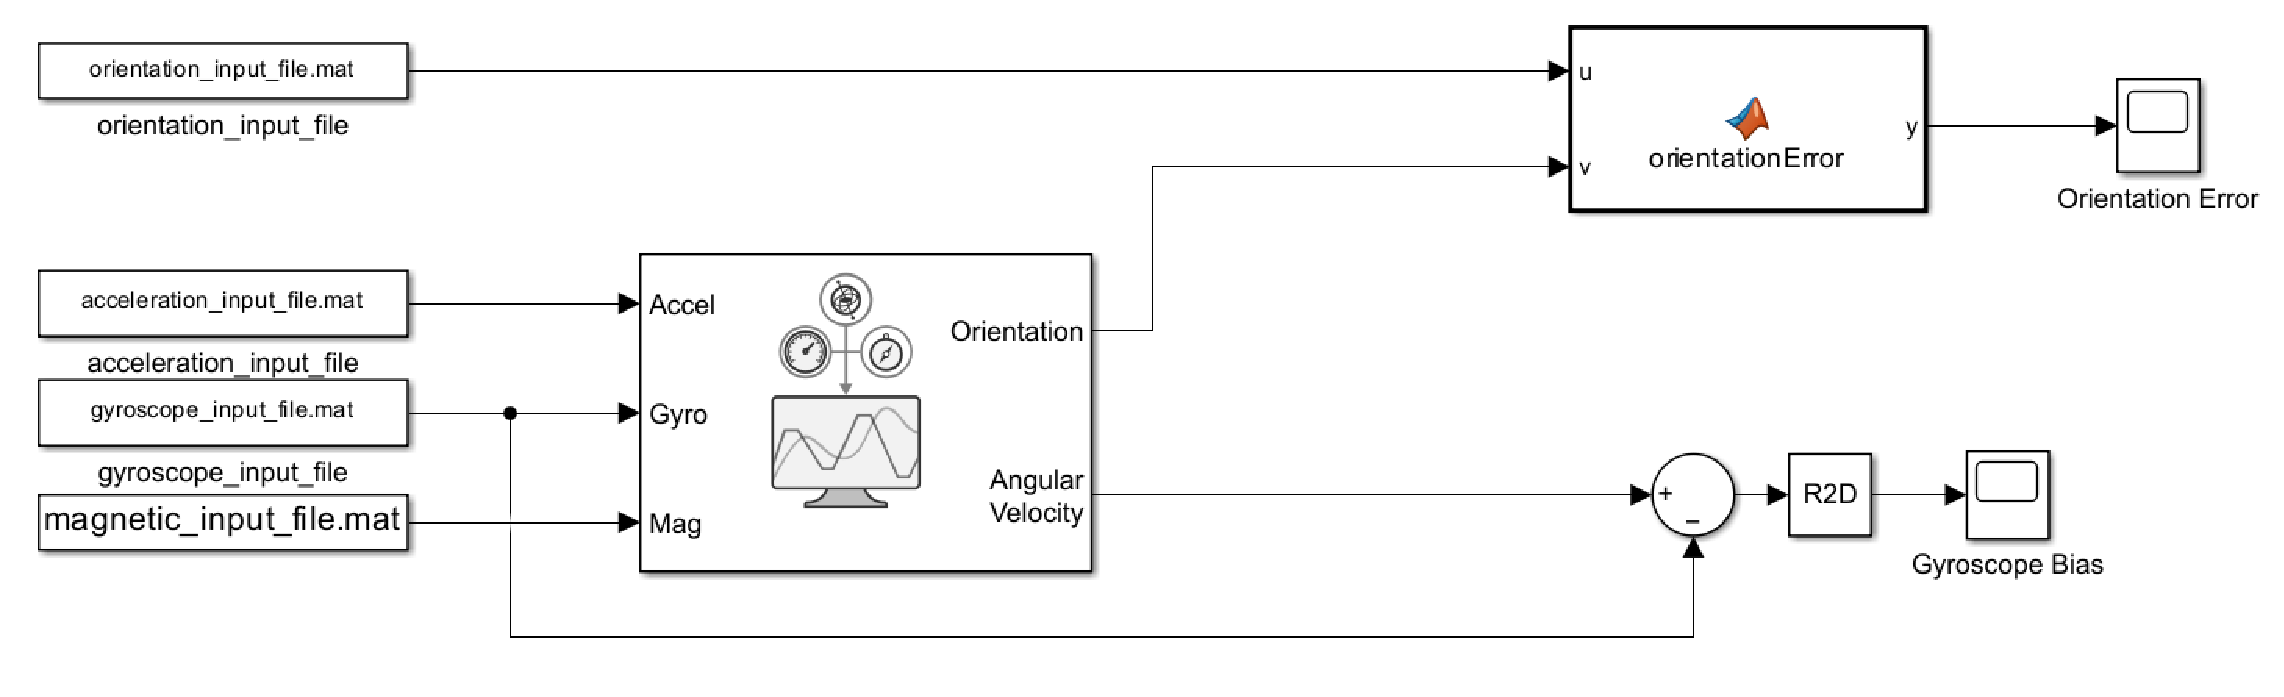
\includegraphics[width=0.8\textwidth]{fig/Capitulo5/Caso_de_estudio_IMU/Generador_de_salidas/flujo_lector_de_archivos.pdf}
    \caption{Diagrama utilizado para la interpretación de los archivos \cite{mathworks2024imu}}
    \label{fig:caso_de_estudio_2_IMU_interpretacion_de_archivos}
\end{figure}


Una vez establecido el diagrama que se encarga de la generación de los datos, en esta sección se explicaran los bloques requeridos para la construcción del diagrama de la Figura \ref{fig:caso_de_estudio_2_IMU_interpretacion_de_archivos}.

\begin{figure}[htbp]
    \centering
    \begin{subfigure}[b]{0.35\textwidth}
        \centering
        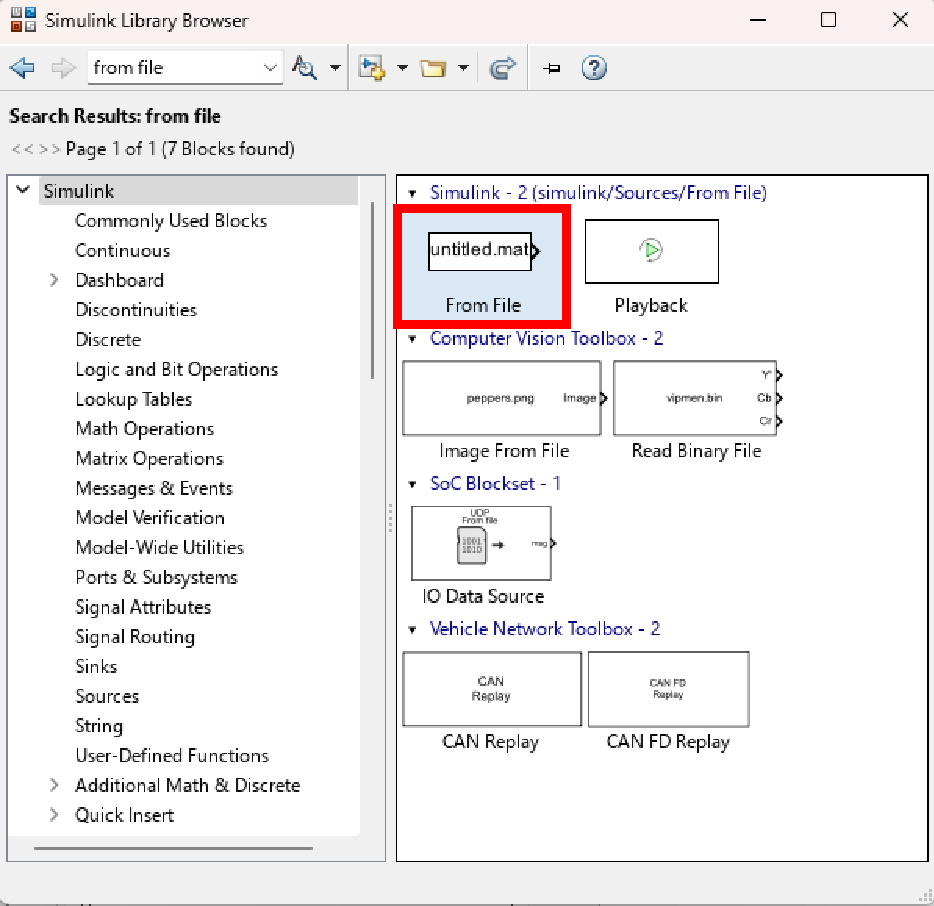
\includegraphics[width=\textwidth]{fig/Capitulo5/Caso_de_estudio_IMU/Generador_de_salidas/libreia_de_bloques_from_file.pdf}
        \caption{Librería de bloques - Leer de archivo}
        \label{fig:lib_bloques_from_file_IMU}
    \end{subfigure}
    \hfill
    \begin{subfigure}[b]{0.45\textwidth}
        \centering
        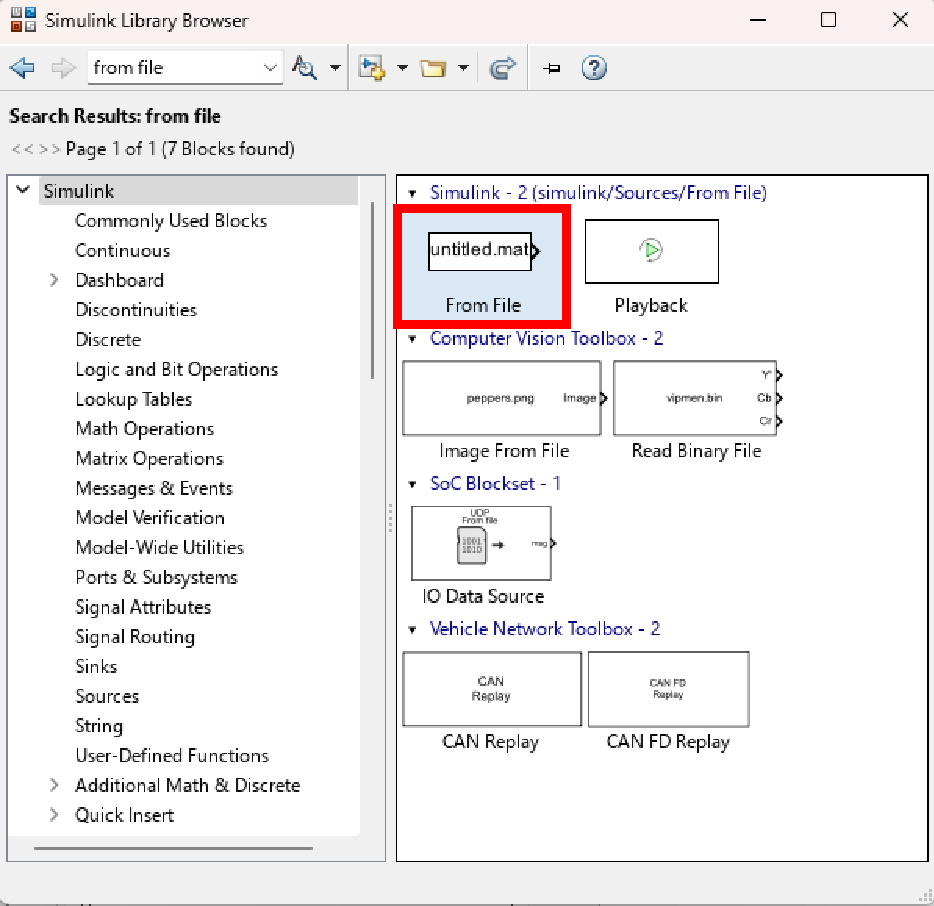
\includegraphics[width=\textwidth]{fig/Capitulo5/Caso_de_estudio_IMU/Generador_de_salidas/libreia_de_bloques_from_file.pdf}
        \caption{Configuración del bloque encargado de la lectura de archivos}
        \label{fig:config_from_file_IMU}
    \end{subfigure}
    \caption{Bloque para la lectura de archivos}
    \label{fig:read_from_file}
\end{figure}

Como mencionamos anteriormente en el desarrollo de este capítulo, en \ref{subsub:generación_de_archivos} se tuvo como salida del programa una serie de archivos generados. Para poder leer los archivos generados previamente se debe de hacer uso del bloque que se muestra en la Figura \ref{fig:read_from_file}, para el correcto funcionamiento del sistema es muy importante que los parámetros de configuración que se muestran en la Figura \ref{fig:config_from_file_IMU}.
\newpage

\begin{figure}[htbp]
    \centering
    % Primera imagen
    \begin{subfigure}[b]{0.35\textwidth}
        \centering
        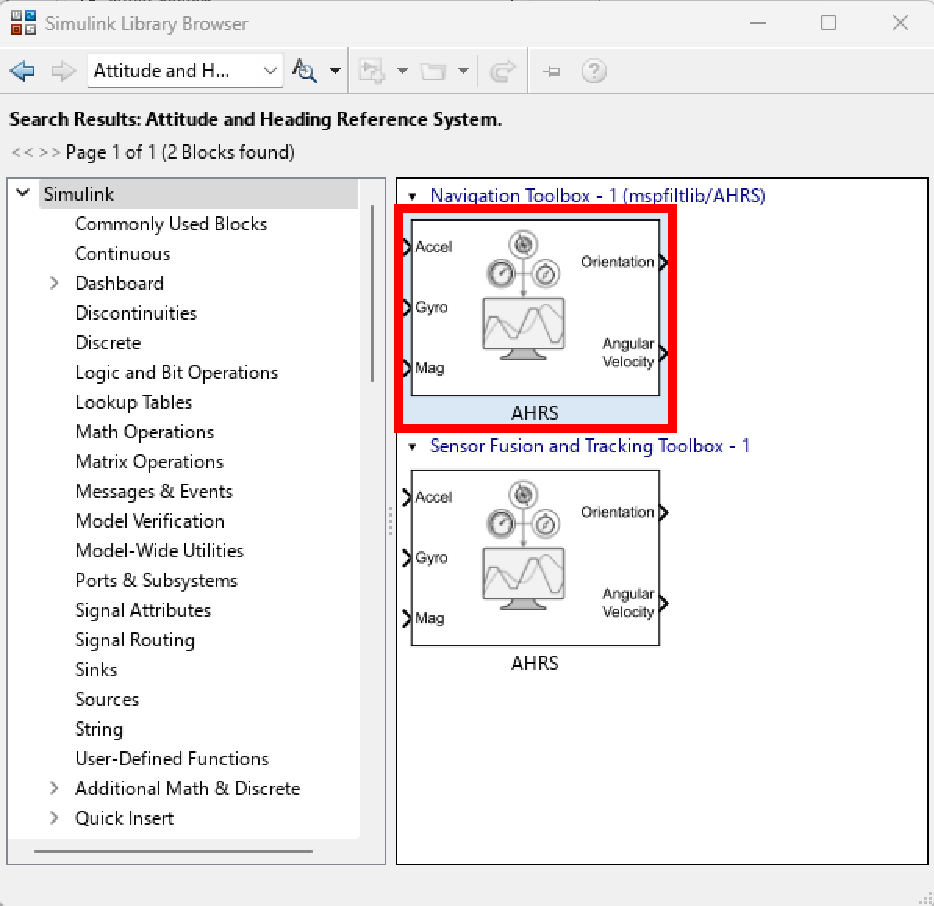
\includegraphics[width=\textwidth]{fig/Capitulo5/Caso_de_estudio_IMU/Generador_de_salidas/libreira_de_bloques_sensor_AHRS.pdf}
        \caption{Librería de bloques - AHRS}
        \label{fig:lib_bloques_AHRS}
    \end{subfigure}
    \hfill
    % Segunda imagen
    \begin{subfigure}[b]{0.45\textwidth}
        \centering
        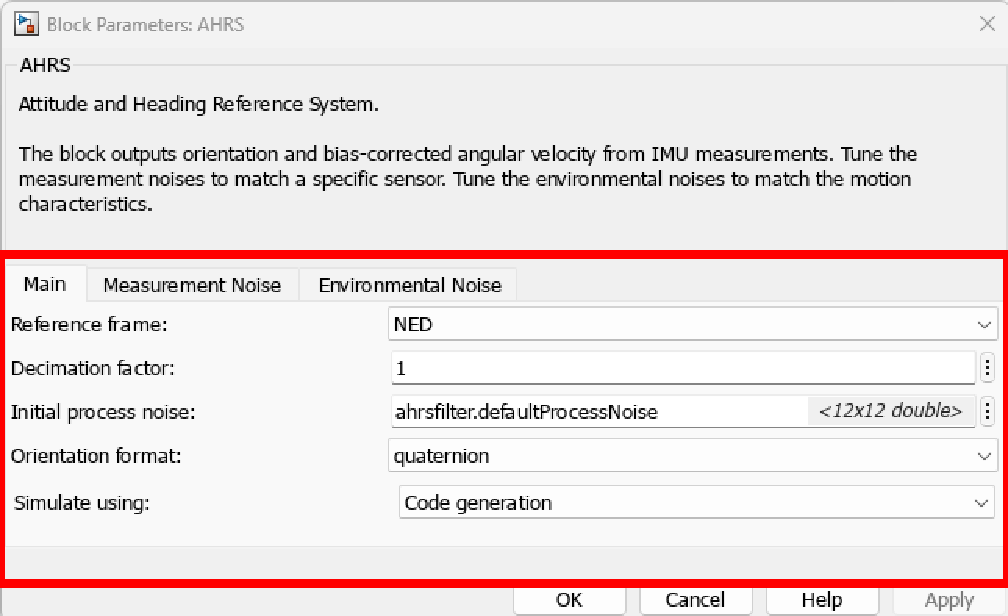
\includegraphics[width=\textwidth]{fig/Capitulo5/Caso_de_estudio_IMU/Generador_de_salidas/configuracion_AHRS_01.pdf}
        \caption{Configuración de parámetros 1}
        \label{fig:parametros_AHRS_01}
    \end{subfigure}
    \hfill
    % Tercera imagen
    \begin{subfigure}[b]{0.45\textwidth}
        \centering
        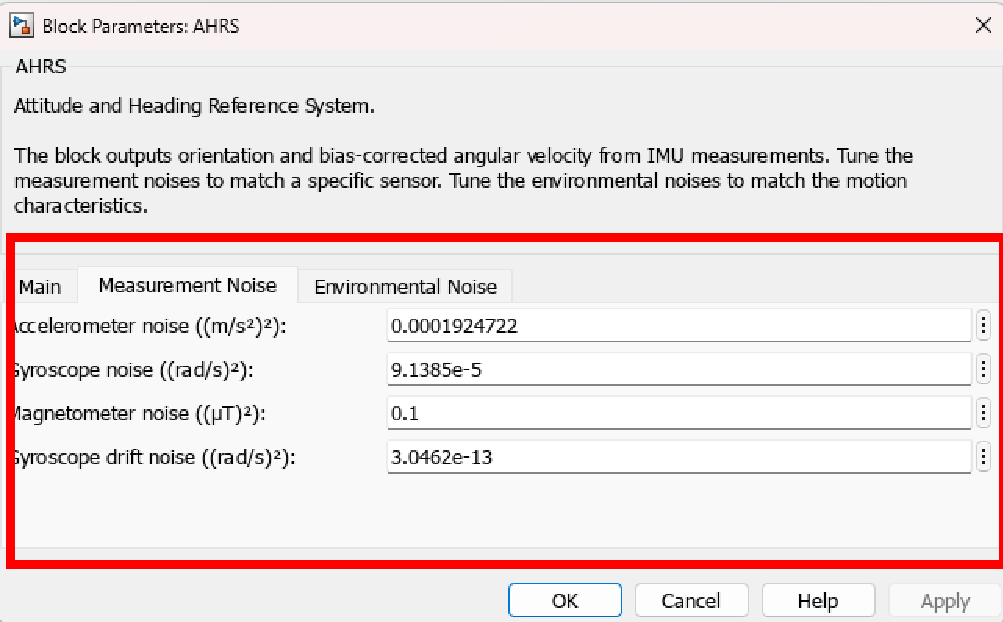
\includegraphics[width=\textwidth]{fig/Capitulo5/Caso_de_estudio_IMU/Generador_de_salidas/configuracion_AHRS_02.pdf}
        \caption{Configuración de parámetros 2}
        \label{fig:parametros_AHRS_02}
    \end{subfigure}
    \hfill
    % Cuarta imagen
    \begin{subfigure}[b]{0.45\textwidth}
        \centering
        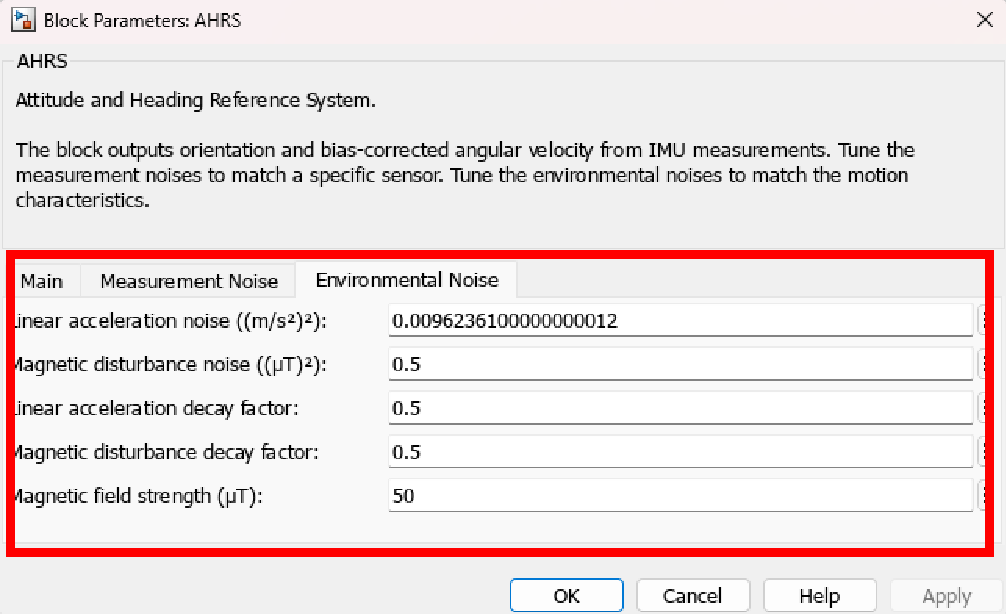
\includegraphics[width=\textwidth]{fig/Capitulo5/Caso_de_estudio_IMU/Generador_de_salidas/configuracion_AHRS_03.pdf}
        \caption{Configuración de parámetros 3}
        \label{fig:parametros_AHRS_03}
    \end{subfigure}

    \caption{Bloque para la simulación del comportamiento de la IMU}
    \label{fig:arreglo_AHRS}
\end{figure}

En la Figura \ref{fig:arreglo_AHRS}, podemos encontrar el bloque denominado AHRS, este es un sistema que proporciona la estimación de la actitud y orientación de un objeto en 3D., es por esto que se debe de seguir una serie de configuraciónes con el objetivo de lograr el correcto funcionamiento del módulo. Su principal función es calcular la orientación del objeto usando datos de sensores como acelerómetros, giroscopios y magnetómetros. Por un lado en la Figura \ref{fig:lib_bloques_AHRS}, podemos observar el nombre del módulo en la Liberia de bloques. Una vez dentro de los parámetros de configuración del bloque tenemos en la Figura \ref{fig:parametros_AHRS_01}, los parámetros principales de configuración, seguido de esto en la Figura \ref{fig:parametros_AHRS_02}, tenemos los parámetros encargados del ruido de la medicion. Finalmente en la Figura \ref{fig:parametros_AHRS_03} se configuran los parametros relacionados al ruido del ambiente. 
\newpage

\begin{figure}[htbp]
    \centering
    \begin{subfigure}[b]{0.35\textwidth}
        \centering
        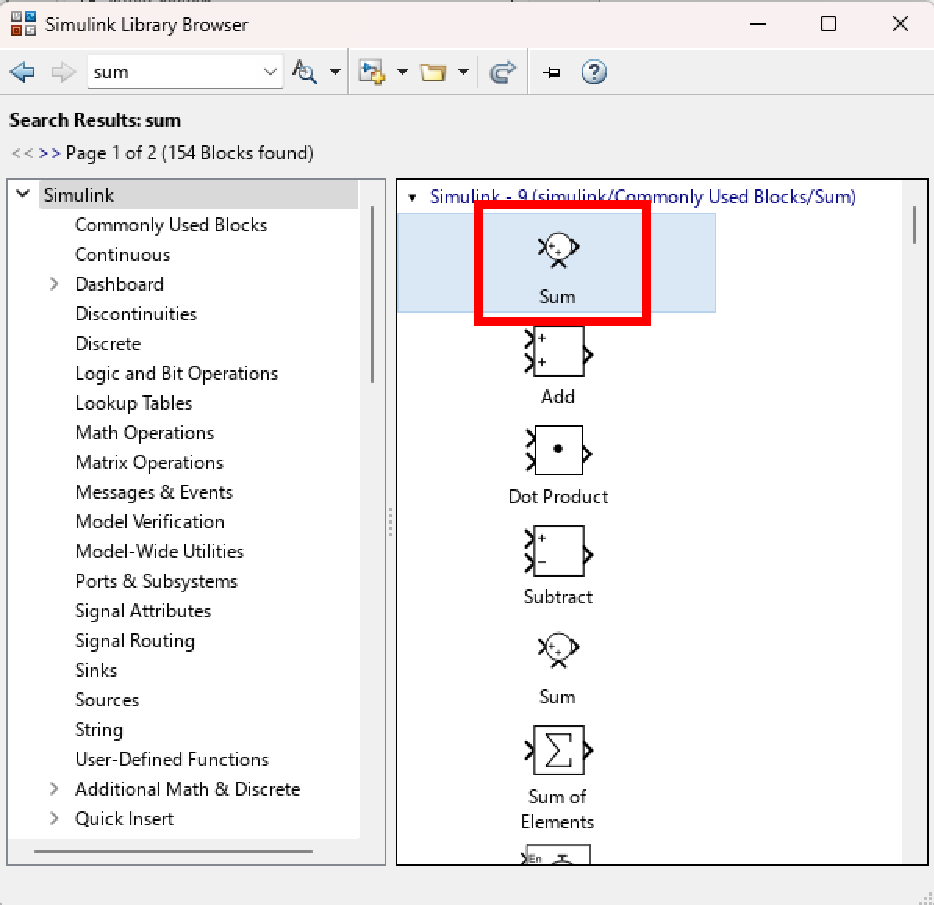
\includegraphics[width=\textwidth]{fig/Capitulo5/Caso_de_estudio_IMU/Generador_de_salidas/libreia_de_bloques_suma.pdf}
        \caption{Librería de bloques - Suma}
        \label{fig:lib_bloques_add_IMU}
    \end{subfigure}
    \hfill
    \begin{subfigure}[b]{0.45\textwidth}
        \centering
        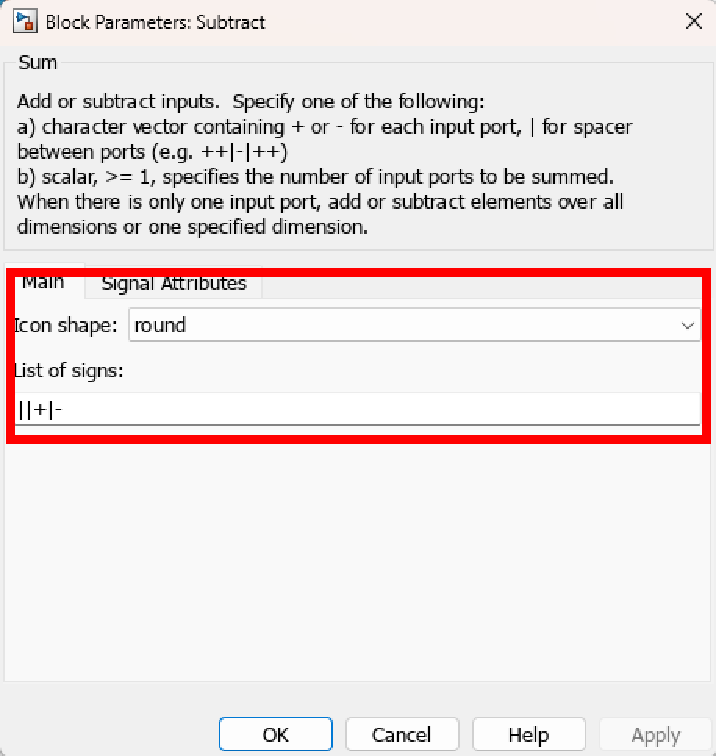
\includegraphics[width=\textwidth]{fig/Capitulo5/Caso_de_estudio_IMU/Generador_de_salidas/configuracion_bloque_suma.pdf}
        \caption{Configuración del bloque encargado de la suma de señales}
        \label{fig:config_add_IMU}
    \end{subfigure}
    \caption{Bloque para la suma de señales}
    \label{fig:add_of_some_signals}
\end{figure}

Para realizar una resta de senales se utiliza el bloque suma , el mismo se puede observar en la Figura \ref{fig:add_of_some_signals}. Se debe de realizar la diferencia con el objetivo de poder calcular la desviación del giroscopio y de esta forma generar un arhcivo de salida con estos datos. 


\begin{figure}[htbp]
    \centering
    \begin{subfigure}[b]{0.35\textwidth}
        \centering
        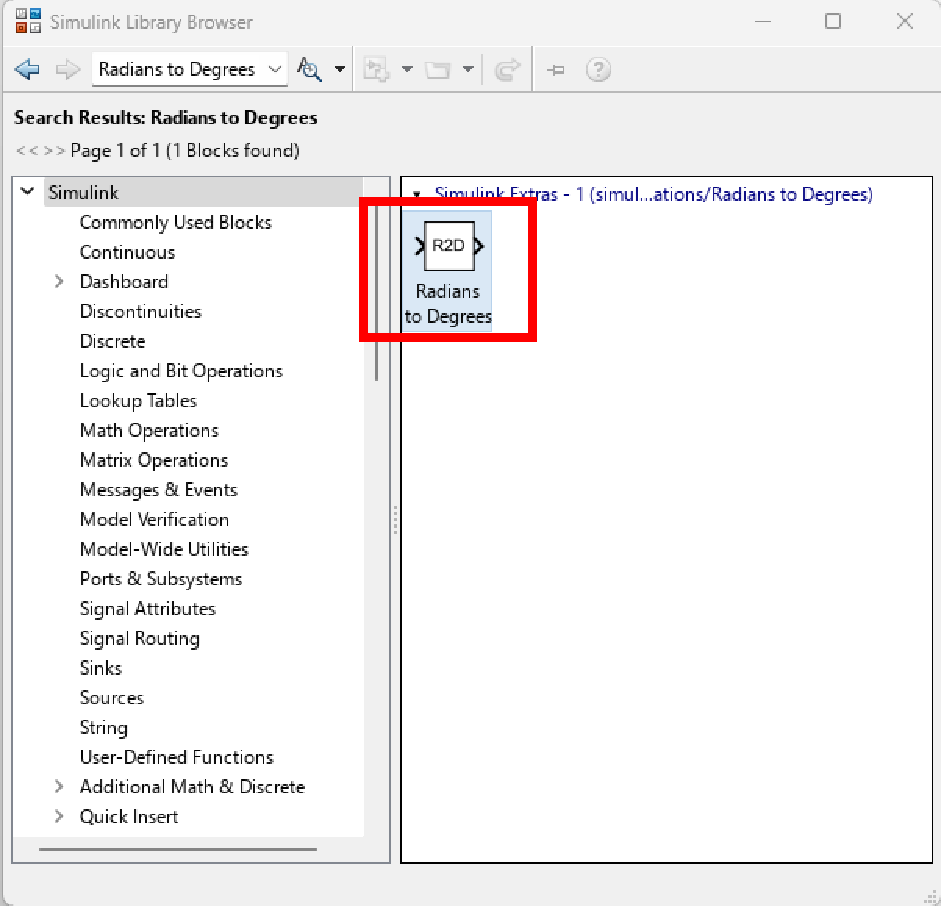
\includegraphics[width=\textwidth]{fig/Capitulo5/Caso_de_estudio_IMU/Generador_de_salidas/libreria_bloque__rad_2_deg.pdf}
        \caption{Librería de bloques - Conversor de radianes a grados}
        \label{fig:lib_bloques_R2D}
    \end{subfigure}
    \hfill
    \begin{subfigure}[b]{0.45\textwidth}
        \centering
        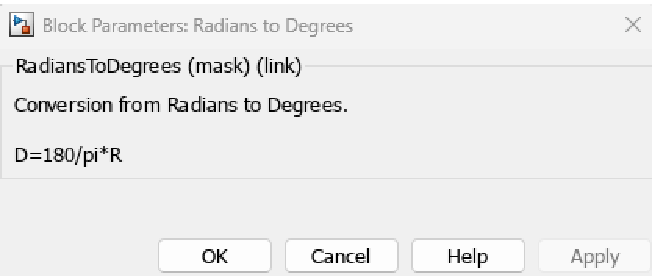
\includegraphics[width=\textwidth]{fig/Capitulo5/Caso_de_estudio_IMU//Generador_de_salidas/configuracion_rad_2_deg.pdf}
        \caption{Configuración del bloque conversor de radianes a grados}
        \label{fig:conf_bloques_R2D}
    \end{subfigure}
    \caption{Bloque para convertir de Radianes a grados}
    \label{fig:bloques_R2D}
\end{figure}

Los bloques de MATLAB trabajan utilizando las medidas de los ángulos en unidades de radianes, es por esto que se utiliza un bloque de trasnformacion para poder obtener los resultados en grados y que sean mas sencillos de interpretar tanto en los datos de salida como en los graficos a elaborar.

\newpage

\begin{figure}[htbp]
    \centering
    \begin{subfigure}[b]{0.35\textwidth}
        \centering
        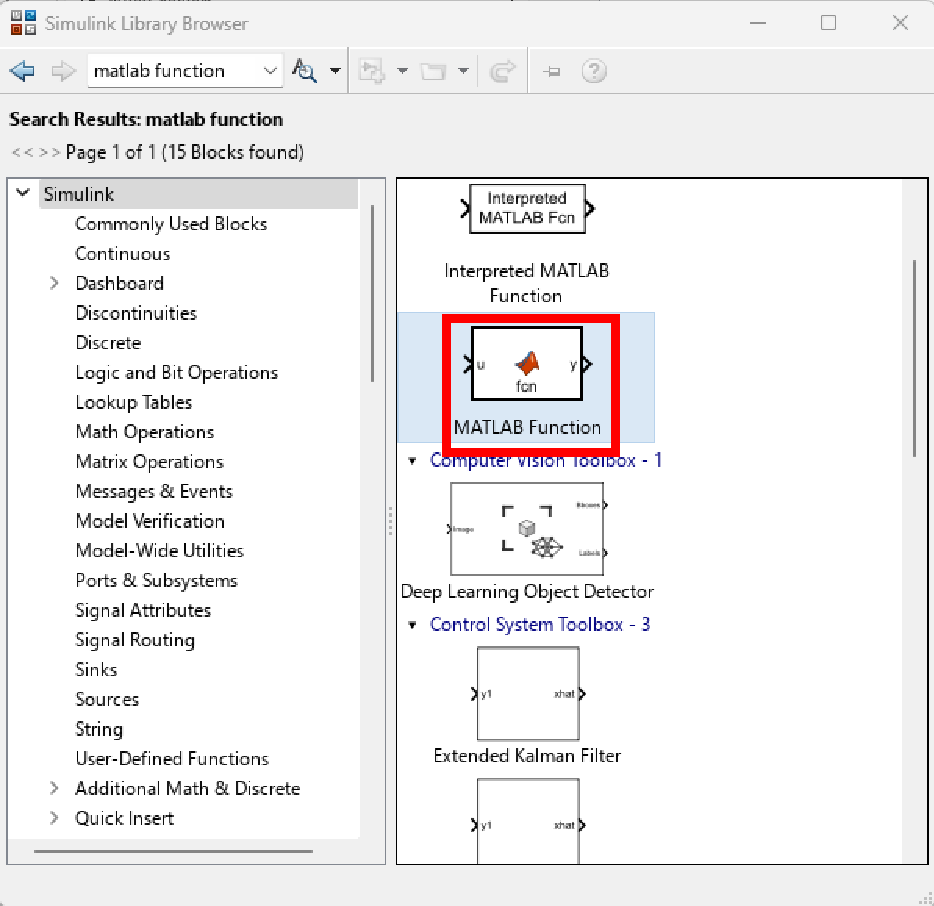
\includegraphics[width=\textwidth]{fig/Capitulo5/Caso_de_estudio_IMU/Generador_de_salidas/libreria_bloque_de_funcion.pdf}
        \caption{Librería de bloques - Función}
        \label{fig:lib_bloques_func}
    \end{subfigure}
    \hfill
    \begin{subfigure}[b]{0.45\textwidth}
        \centering
        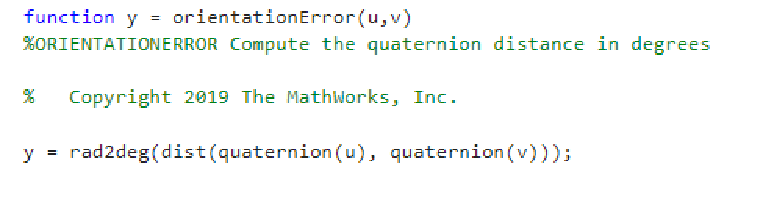
\includegraphics[width=\textwidth]{fig/Capitulo5/Caso_de_estudio_IMU/Generador_de_salidas/configuracion_codigo.pdf}
        \caption{Configuración del bloque de Función}
        \label{fig:config_bloques_func}
    \end{subfigure}
    \caption{Bloque para aplicar una función implementada mediante código}
    \label{fig:bloques_func}
\end{figure}

Finalmente se implementa un bloque de código el cual se encarga de calcular el error de orientación del sistema esto con el fin de estimar la precisión con la cual el gisrocopio simualdo en este caso de estudio puede determinar la orientacion, en la Figura \ref{fig:lib_bloques_func} se puede observar el bloque en la libreria, seguido de esto en la Figura \ref{fig:config_bloques_func} se puede observar el código implementado dentro de este bloque. El archivo se debera de guardar bajo el nombre de (IMUFusionSimulinModel) y el tiempo de ejecucio se debe de establecer en 1000ms. 
\newpage

\subsection{Resultados de la simulación}\label{subsub:resultados_simulados_IMU}

\begin{figure}[htbp]
    \centering
    % Imagen superior
    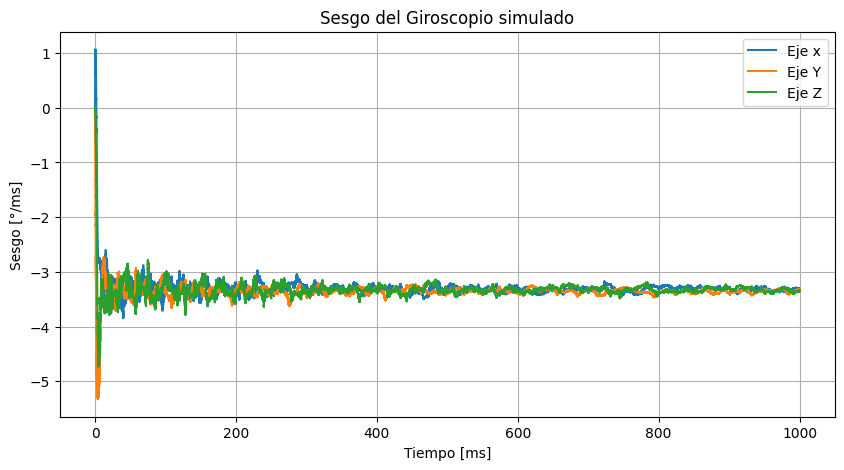
\includegraphics[scale=0.3]{fig/Capitulo5/Caso_de_estudio_IMU/data/simulated/sesgo_simulado.png}
    % Espacio entre las imágenes (opcional)
    \vspace{1cm}
    % Imagen inferior
    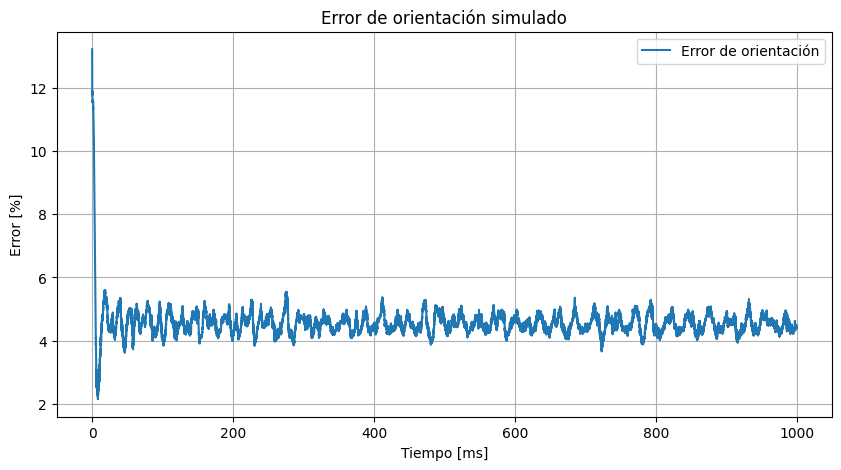
\includegraphics[scale=0.3]{fig/Capitulo5/Caso_de_estudio_IMU/data/simulated/error_de_orientacion_simulado.png}
    \caption{Datos simulados}
    \label{fig:data_simulated}
\end{figure}

Ejecutando el sistema en el entorno de simulacion MATLAB Simulink se obtienen los resutlados que se muestran en \ref{fig:data_simulated}, al lado izquierdo se pueden observar los datos de la desviacion simulada del sistema mientras que al lado derecho se observan los datos correspondientes a error de orientacion. Cabe estacar que el resultado es esperado ya que la diferencia entre la orientación estimada y la verdadera debería ser casi 4.7 [grados], que es la declinación en esta latitud y longitud y en el bloque IMU, al giroscopio se le dio una polarización de 0,0545 [rad/s] o 3,125 [grados/s], que debería coincidir con el valor de estado estacionario. En las proximas secciónes se detallaran los pasos a seguir para la implementacion de este sistema en la tarjeta de desarrollo por medio del flujo de trabajo desarrollado en en capitulo \ref{ch:especifico2}. 

\newpage

\subsection{Implementación en la Tarjeta de desarrollo mediante EmbedSynthGNC}


Para la implementación en la tarjeta de desarrollo ZedBoard se ejecuta el flujo de trabajo que se muestra en la sección \ref{sec:m2m_transformator}. El mismo es representado mediante el diagrama que se muestra en la Figura \ref{fig:m2m_matlab_simulink_coder}.

Primeramente se deben de generar los archivos de Codigo C desde MATLAB Simulink, para esto se deben de seguir el diagrama de la Figura \ref{fig:m2m_matlab_simulink_coder}. 

\begin{figure}[h!]
    \centering
    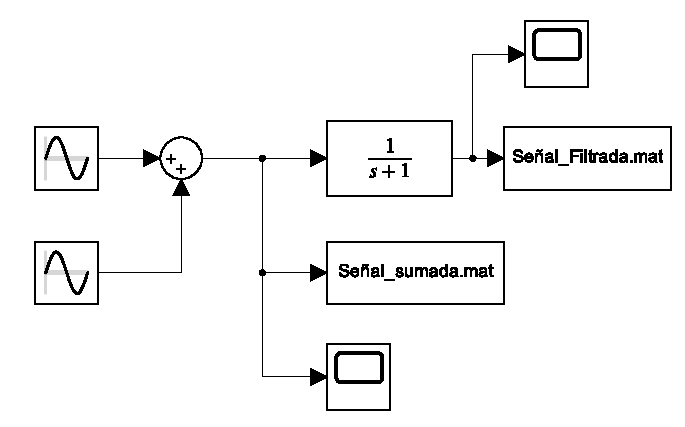
\includegraphics[width=0.5\textwidth]{fig/especifico_2/CASO_ESTUDIO_FILTRO/Diagrama matlab simulink scope.pdf}
    \caption{Definicion del tiempo de ejecucion del sistema}
    \label{fig:system_runtime_IMU}
\end{figure}

Como primer punto se deben realizar las configraciones que se muestran en la Figura \ref{fig:system_runtime_IMU} donde se debe de definir el tiempo de ejecucion del sistema, para este caso se selecciona una ejecucion de 1000 ms, esto debido a que mediante mediciones se logra determinar que el bloque se estabiliza a los 1000ms de ejecucion. 

\begin{figure}[h!]
    \centering
    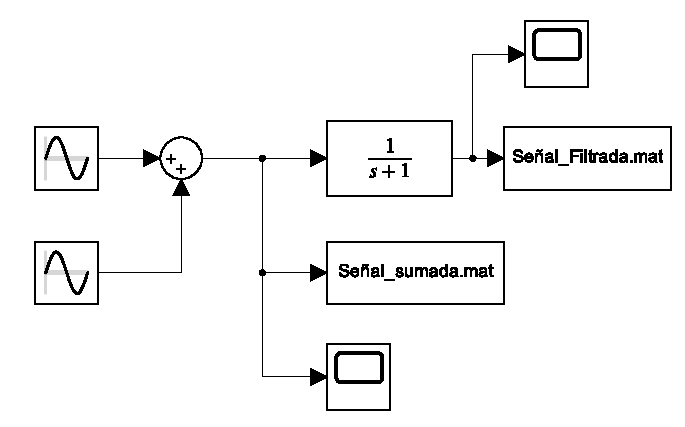
\includegraphics[width=0.5\textwidth]{fig/especifico_2/CASO_ESTUDIO_FILTRO/Diagrama matlab simulink scope.pdf}
    \caption{Definicion del procesador objetivo y arquitectura}
    \label{fig:system_target_IMU}
\end{figure}

Seguido de esto como se muestra en la Figura \ref{fig:system_target_IMU} se debe de establecer el procesador objetivo y la arquitectura del mismo.Finalmente se debe de definir el tipo de archivo de construccion el cual se puede observar en la Figura \ref{fig:pestana_config_output_file}. 

El archivo resultante sera un archivo llamado IMUFusionSimulinModel.zip seguido de esto se debe de  se exportan los archivos al sistema Linux. Una vez exportados los archivos se descomprimen los mismos en la carpeta denominada swap area.

\begin{figure}[h!]
    \centering
    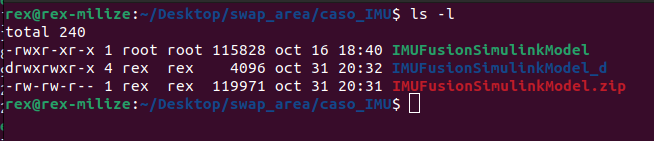
\includegraphics[width=0.5\textwidth]{fig/Capitulo5/Caso_de_estudio_IMU/retornos_consola/Screenshot from 2024-10-31 20-33-27.png}
    \caption{Archivo de construcción en el directorio swap area}
    \label{fig:swap_area_imu}
\end{figure}

\begin{lstlisting}[language=bash, caption={Compilacion del programa , Linux}, label=lst:build_cmake_file_IMU]
    cmake -DCMAKE_C_COMPILER=arm-linux-gnueabihf-gcc 
    CMakeLists.txt -DMATLAB_ROOT=/home/test/IMUFusionSimulinModel/R2024b/
\end{lstlisting}

Una vez descomprimidos los archivos en el directorio denominado como swap area se deben enviar al container mediante el comadno que se muestra en \ref{fig:swap_area_imu}. Una vez dentro del contenedor se debe construir el archivo responsable de la compilacion del codigo C, esto se logra mediante el comando que se muestra en \ref{lst:build_cmake_file_IMU}. El archivo binario resultante se encuentra en la ruta /home/IMUFusionSimulinModel/IMURAW, el mismo se debe de enviar al directorio denominado swap area, este se debe de exportar al contenedor encargado de integrarlo a la imagen generada mediante el marco de trabajo de Yocto y el flujo de trabajo de EmbedSynthGNC. 


Una vez dentro del contendor se debe de ir al directorio denominado meta-EmbedSynthGNC dentro del mismo se debe ingresar a la ruta /poky/meta-EmbedsinthGNC/recipes-core y en la misma se debe agregar un directorio con el nombre de (imu). Ademas de esto se debe inicializar el ambiente de trabajo mediante el uso del comando \ref{lst:yocto_ambient_set}. Una vez inicializado el ambiente de trabajo se debe agregar la nueva capa generada al archivo deniminado local.conf esto con el fin que el binario con el nombre IMUFusionSimulinModel sea incluido en la generación de la imagen. Una vez generada la imagen se deben repetir los pasos que se muestran en \ref{sub:image2zedboard} donde se contempla exportar los archivos contenidos en la ruta xxxxx. Seguido de esto se debe preparar la memoria extraible de la tarjeta de desarrollo para los nuevos archivos.

\newpage

\subsection{Resultados de la implementación}

\begin{figure}[htbp]
    \centering
    \begin{subfigure}[b]{0.35\textwidth}
        \centering
        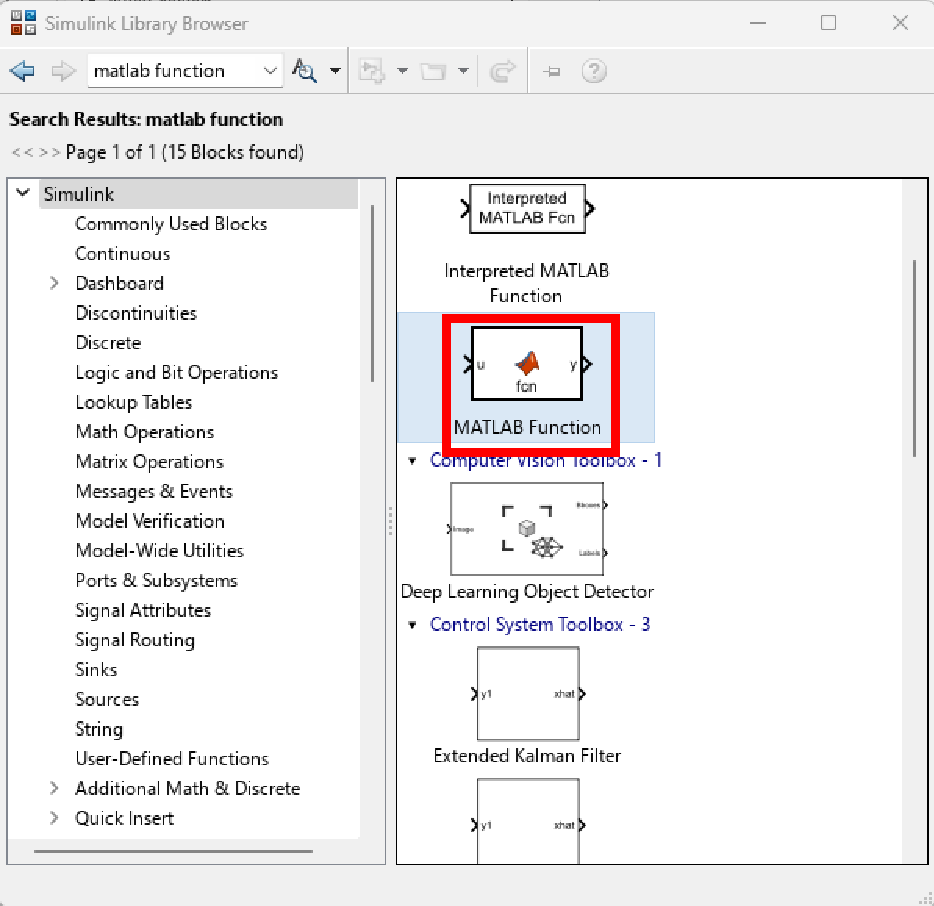
\includegraphics[width=\textwidth]{fig/Capitulo5/Caso_de_estudio_IMU/Generador_de_salidas/libreria_bloque_de_funcion.pdf}
        \caption{Tarjeta de desarrollo ZedBoard - IMU}
        \label{fig:imu_zedboard}
    \end{subfigure}
    \hfill
    \begin{subfigure}[b]{0.45\textwidth}
        \centering
        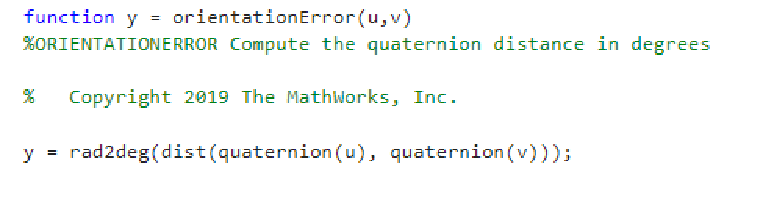
\includegraphics[width=\textwidth]{fig/Capitulo5/Caso_de_estudio_IMU/Generador_de_salidas/configuracion_codigo.pdf}
        \caption{Archivos de salida}
        \label{fig:out_files_IMU}
    \end{subfigure}
    \caption{Programa IMUFusionSimulinModel implementado en la tarjeta de desarrollo}
    \label{fig:IMU_ZEDBOARD}
\end{figure}
Como se puede observar en la Figura \ref{fig:imu_zedboard} se observa el binario contenido en la imagen dentro de la tarjeta de desarrollo. Una vez ejecutado el mismo se obtienen los archivos de salida que se muestran en la Figura \ref{fig:out_files_IMU}. 

\begin{figure}[htbp]
    \centering
    \begin{subfigure}[b]{0.35\textwidth}
        \centering
        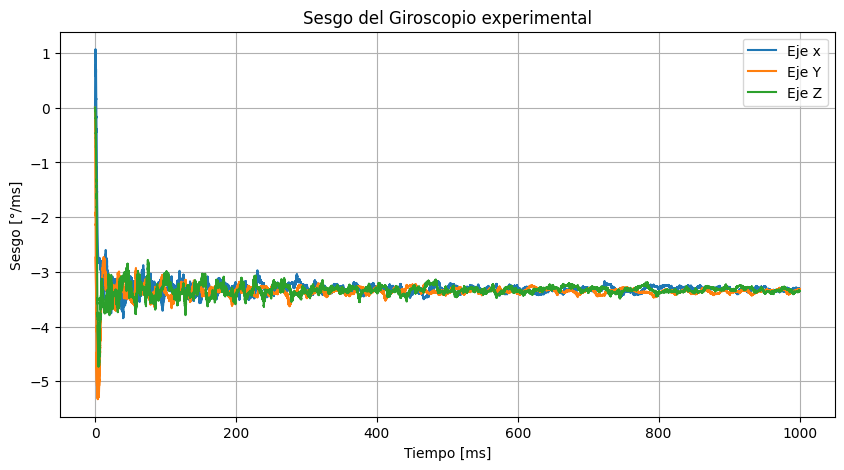
\includegraphics[width=\textwidth]{fig/Capitulo5/Caso_de_estudio_IMU/data/experimental/sesgo_experimental.png}
        \caption{Sesgo del giroscopio experimental}
        \label{fig:imu_sesgo_exp}
    \end{subfigure}
    \hfill
    \begin{subfigure}[b]{0.45\textwidth}
        \centering
        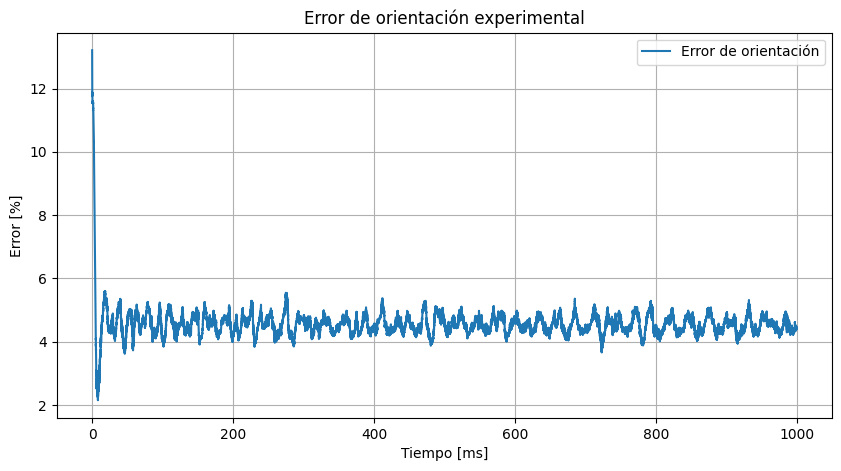
\includegraphics[width=\textwidth]{fig/Capitulo5/Caso_de_estudio_IMU/data/experimental/error_de_orientacion.png}
        \caption{Error de orientación experimental}
        \label{fig:out_files_IMU_eo_exp}
    \end{subfigure}
    \caption{Datos de archivo de salida IMU}
    \label{fig:IMU_ZEDBOARD_exp}
\end{figure}

Analizando los mismos mediante el programa de Python \ref{apx:comparacion_de_sennales_programa} se obtienen los graficos que se muestran en \ref{fig:IMU_ZEDBOARD_exp}, en donde a la izquierda en la Figura \ref{fig:imu_sesgo_exp} se muestra el grafico relacionado al sesgo del giroscopio en sus 3 ejes de operacion, a la derecha en la Figura \ref{fig:out_files_IMU_eo_exp} se muestra el grafico de error de operacion del giroscopio. Realizando la comparacion con los datos simulados obtenidos en \ref{subsub:resultados_simulados_IMU}, se obtienen los siguientes resultados para el analisis de error.

Para la desviación del eje X


\begin{itemize}
    \item Error Promedio Absoluto = $2.31 \times 10^{-15}$ []
    \item Error Cuadrático Medio = $3.09 \times 10^{-15}$ $[^{2}]$
    \item Raíz del Error Cuadrático Medio = $9.56 \times 10{-30}$ []
\end{itemize}

Para la desviación del eje Y


\begin{itemize}
    \item Error Promedio Absoluto = $2.36 \times 10^{-15}$ []
    \item Error Cuadrático Medio = $3.29 \times 10^{-15}$ $[^{2}]$
    \item Raíz del Error Cuadrático Medio = $1.08 \times 10{-29}$ []
\end{itemize}


Para la desviación del eje Z


\begin{itemize}
    \item Error Promedio Absoluto = $3.19 \times 10^{-15}$ []
    \item Error Cuadrático Medio = $4.58 \times 10^{-15}$ $[^{2}]$
    \item Raíz del Error Cuadrático Medio = $2.10 \times 10{-29}$ []
\end{itemize}


De los cuales se puede determinar que dado el orden de magnitud tan pequeño de los errores en cada eje, las mediciones del giroscopio son altamente precisas, con variaciones mínimas. Las diferencias entre los ejes (ligeramente más altas en el eje Z) podrían deberse a factores menores de calibración o sensibilidad en el giroscopio, pero en general se logra obtener un desempeño excelente.


Por otro lado los datos relacionados al error de orientacion se obtiene que las diferencias mostradas en estas gráficas es dé.


\begin{itemize}
    \item Error Promedio Absoluto = $1.28 \times 10^{-13}$ []
    \item Error Cuadrático Medio = $2.12 \times 10^{-13}$ $[^{2}]$
    \item Raíz del Error Cuadrático Medio = $4.51 \times 10{-26}$ []
\end{itemize}


Aunque los errores en la orientación son de una magnitud algo mayor que en los ejes individuales del giroscopio, siguen siendo muy pequeños. Esto sugiere que el sistema de orientación es muy preciso, aunque hay un pequeño margen de acumulación de error que sería esperado en cálculos de orientación que integran múltiples ejes. 

\newpage

\section{Caso de estudio 3 - PID}

Finalmente como ultimo caso de estudio se desarrolla un controlador PID (Proporcional-Integral-Derivativo) es una herramienta clave en los sistemas de control automático, diseñada para minimizar el error entre una señal de referencia y la señal de salida real. Su importancia radica en su capacidad para ajustar la respuesta del sistema, logrando un equilibrio entre rapidez y estabilidad. Esto permite que el controlador maneje eficazmente perturbaciones y cambios en el entorno, siendo aplicable a una variedad de sistemas, como motores eléctricos, sistemas de calefacción y procesos industriales complejos.

En el contexto de MATLAB y Simulink, estas herramientas ofrecen una plataforma visual que facilita la implementación y ajuste de controladores PID. A través de bloques específicos en Simulink, los ingenieros pueden modificar en tiempo real los parámetros proporcional, integral y derivativo, observando directamente cómo estos ajustes afectan la salida del sistema. Esta capacidad de simulación y diseño iterativo no solo optimiza el rendimiento del sistema controlado, sino que también proporciona un entorno propicio para la experimentación y el aprendizaje práctico en el campo del control automático.


\subsection{Implementación en MATLAB Simulink}

\begin{figure}[h!]
    \centering
    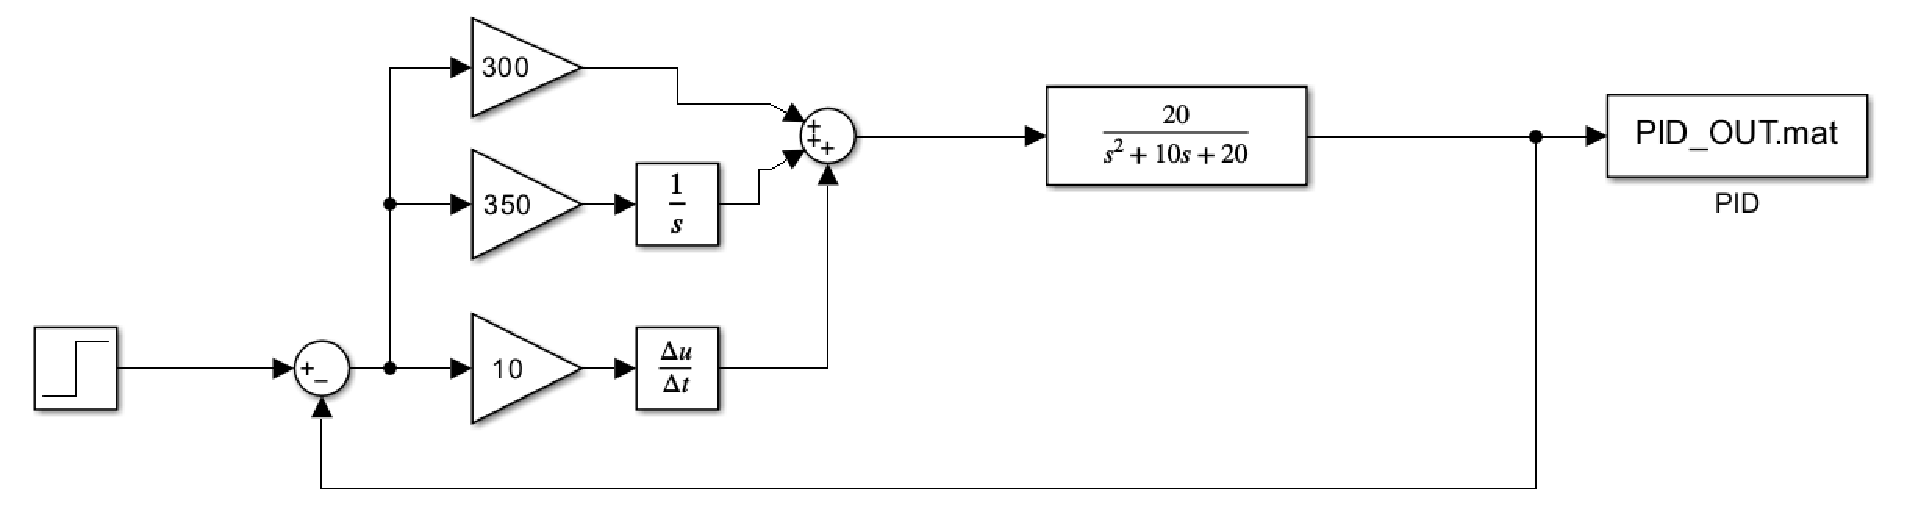
\includegraphics[width=0.8\textwidth]{fig/Capitulo5/Caso_de_estudio_PID/PID_Diagram.pdf}
    \caption{Diagrama completo del caso de estudio 3 - PID }
    \label{fig:caso_de_estudio_3_PID}
\end{figure}


Como se puede observar en la Figura \ref{fig:caso_de_estudio_3_PID}, este es el caso de estudio que se propone en \cite{microcontrollerslab_pid_controller_design}, a este caso de estudio se le deben de realizar unas modificaciones de acuerdo al funcionamiento deseado que se tiene para este caso de estudio, siempre generando datos en el ámbito de simulación en MATLAB para luego contrastar los mismos con los datos obtenidos en la ejecución del modelo en la tarjeta de desarrollo seleccionada.

\subsection{Bloques utilizados para la implementación}

Los bloques utilizados se obtienen en la librería de bloques de MATLAB Simulink. A continuación se muestran los bloques requeridos, asi como la configuración de los mismos para la correcta operación del modelo.

%%step
\begin{figure}[htbp]
    \centering
    \begin{subfigure}[b]{0.35\textwidth}
        \centering
        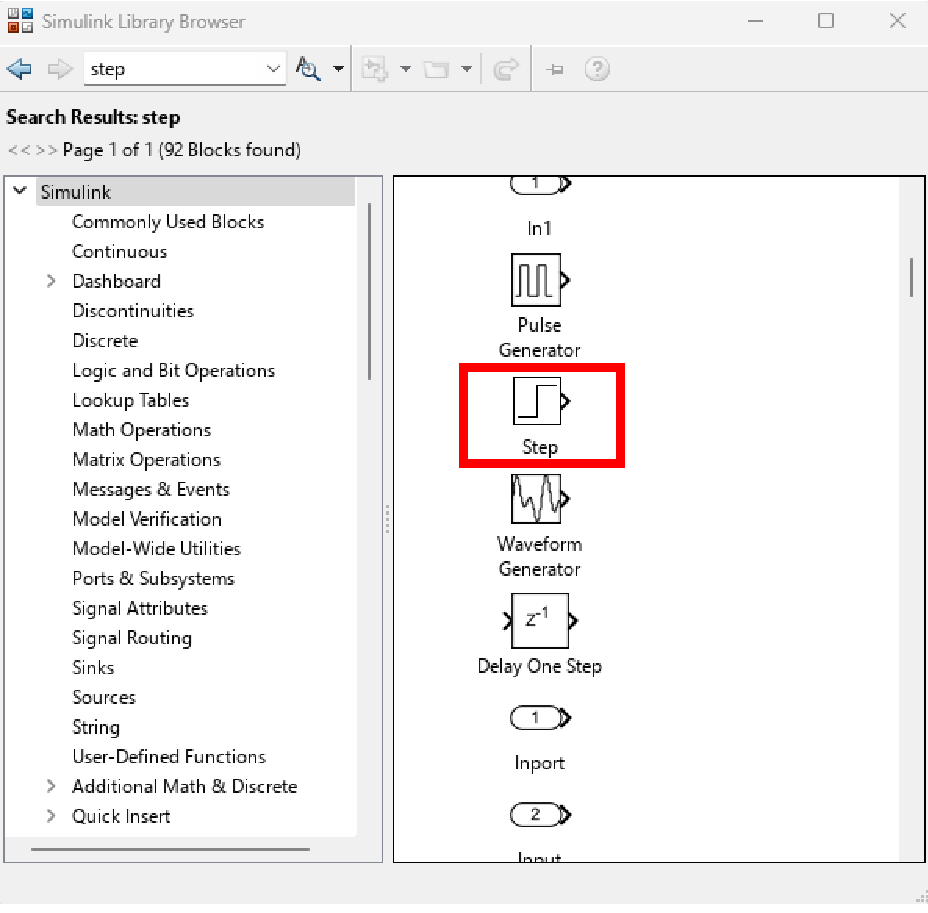
\includegraphics[width=\textwidth]{fig/Capitulo5/Caso_de_estudio_PID/lib_step.pdf}
        \caption{Librería de bloques - Escalon}
        \label{fig:step_lib}
    \end{subfigure}
    \hfill
    \begin{subfigure}[b]{0.45\textwidth}
        \centering
        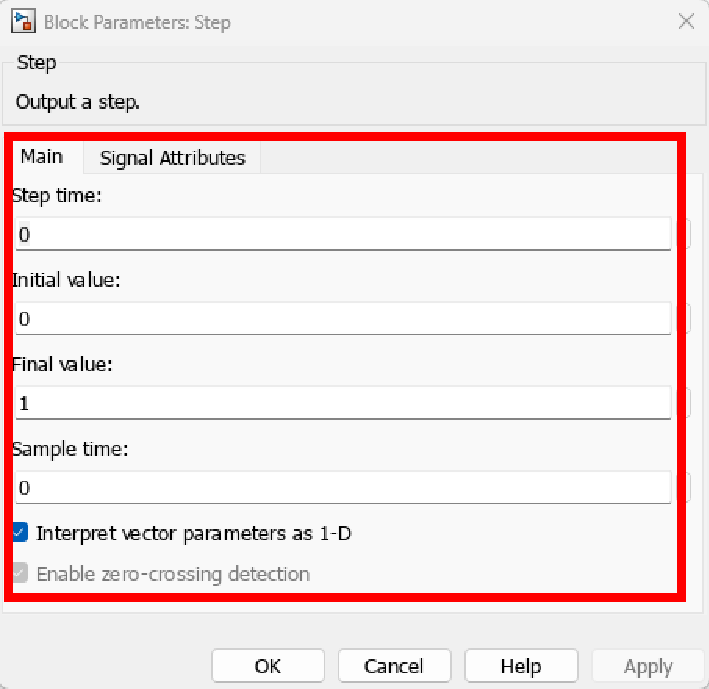
\includegraphics[width=\textwidth]{fig/Capitulo5/Caso_de_estudio_PID/config_step.pdf}
        \caption{Configuración del bloque encargado de generar un escalon }
        \label{fig:step_conf}
    \end{subfigure}
    \caption{Bloque escalon}
    \label{fig:step_block}
\end{figure}
\newpage

Primeramente para la implementación del modelo que se muestra en la Figura \ref{fig:caso_de_estudio_3_PID}, se debe de utilizar el bloque que se muestra en la Figura \ref{fig:step_block}, el mismo se puede encontrar en la libreria de bloques como se muestra en al Figura \ref{fig:step_lib}, ademas de esto la configuracion del mismo se muestra en la Figura \ref{fig:step_conf}.

%%integrator
\begin{figure}[htbp]
    \centering
    \begin{subfigure}[b]{0.35\textwidth}
        \centering
        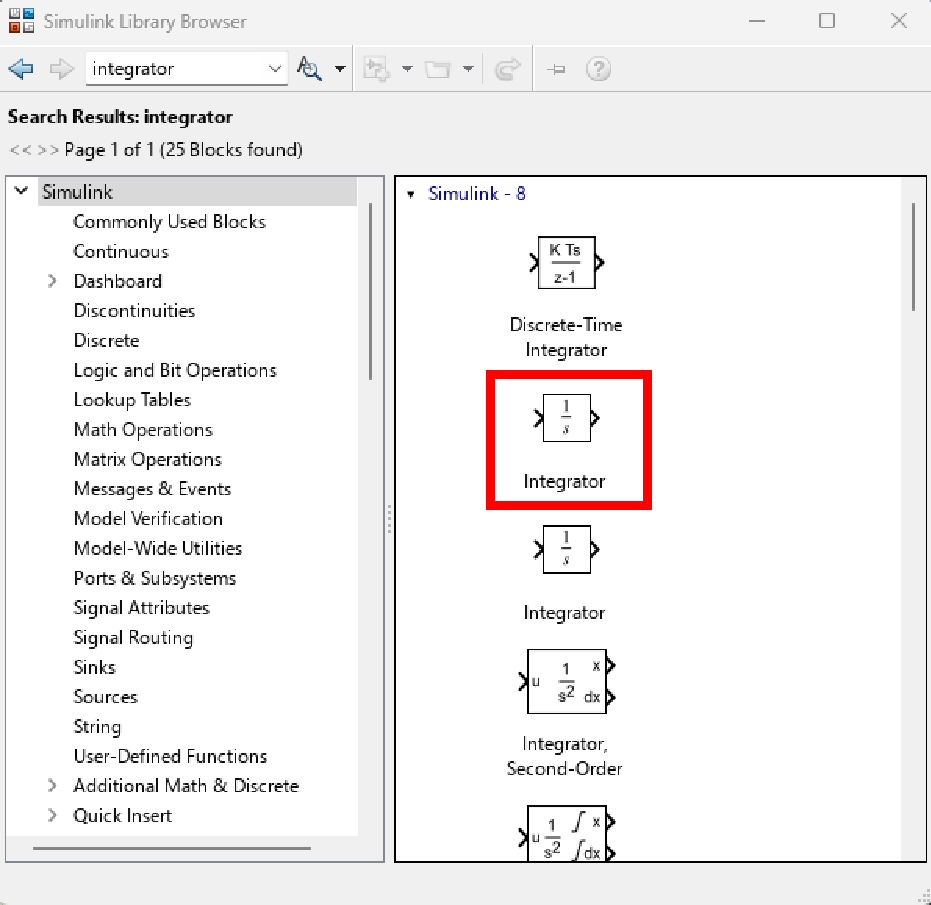
\includegraphics[width=\textwidth]{fig/Capitulo5/Caso_de_estudio_PID/lib_integrator.pdf}
        \caption{Librería de bloques - Integrador}
        \label{fig:int_PID_lib}
    \end{subfigure}
    \hfill
    \begin{subfigure}[b]{0.45\textwidth}
        \centering
        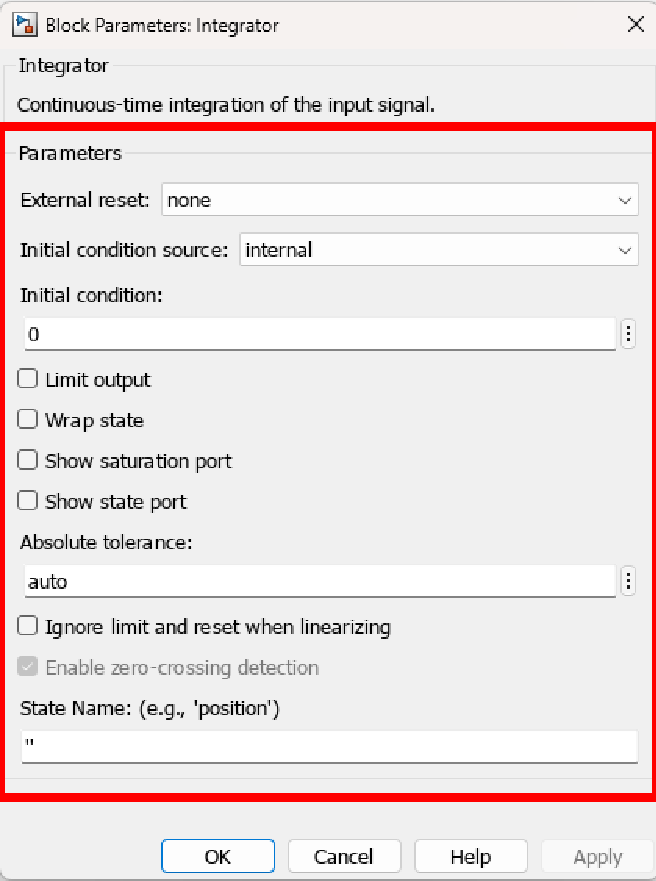
\includegraphics[width=\textwidth]{fig/Capitulo5/Caso_de_estudio_PID/config_integrator.pdf}
        \caption{Configuración del bloque encargado de Integrar}
        \label{fig:int_conf_PID}
    \end{subfigure}
    \caption{Bloque integrador}
    \label{fig:int_block}
\end{figure}

Por un lado, al realizar la implementación del controlador PID por separado se debe de implementar un bloque especializado para la integracion, esto se logra mediante el uso del bloque que se muestra en la Figura \ref{fig:int_block}, el mismo se obtiene de la libreria de bloques como se muestra en la Figura \ref{fig:int_PID_lib}. La configuracion de este bloque se puede observar en la Figura \ref{fig:int_conf_PID}.

\newpage

%%derivative
\begin{figure}[htbp]
    \centering
    \begin{subfigure}[b]{0.35\textwidth}
        \centering
        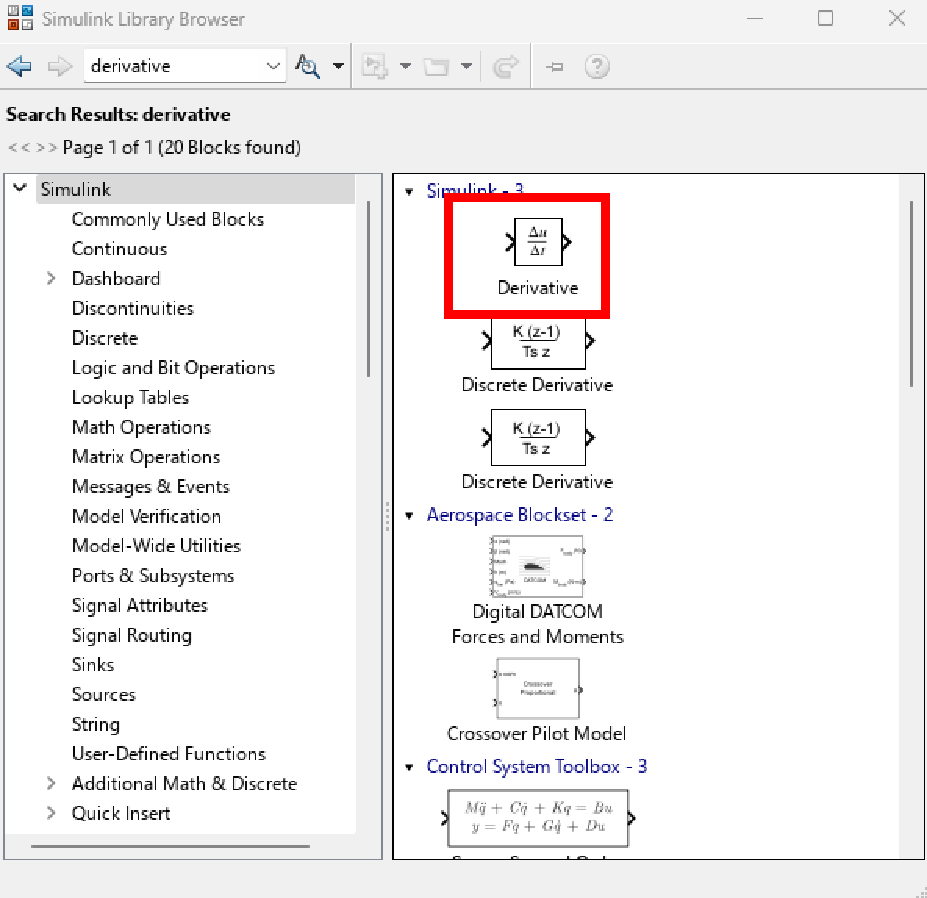
\includegraphics[width=\textwidth]{fig/Capitulo5/Caso_de_estudio_PID/lib_derivative.pdf}
        \caption{Librería de bloques - Derivador}
        \label{fig:dev_PID_lib}
    \end{subfigure}
    \hfill
    \begin{subfigure}[b]{0.45\textwidth}
        \centering
        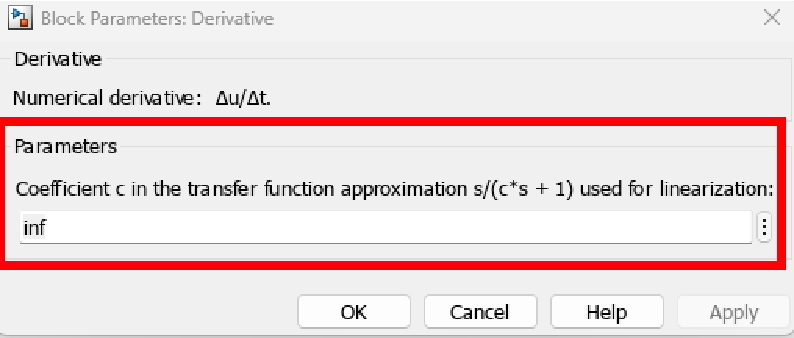
\includegraphics[width=\textwidth]{fig/Capitulo5/Caso_de_estudio_PID/config_derivative.pdf}
        \caption{Configuración del bloque encargado de derivar}
        \label{fig:dev_PID_conf}
    \end{subfigure}
    \caption{Bloque derivador}
    \label{fig:dev_block}
\end{figure}

Por otro lado, tenemos un bloque especializado para la derivacion, esto se logra mediante el uso del bloque que se muestra en la Figura \ref{fig:dev_block}, el mismo se obtiene de la libreria de bloques como se muestra en la Figura \ref{fig:dev_PID_lib}. La configuracion de este bloque se puede observar en la Figura \ref{fig:dev_conf_PID}. 

%%
\begin{figure}[htbp]
    \centering
    \begin{subfigure}[b]{0.35\textwidth}
        \centering
        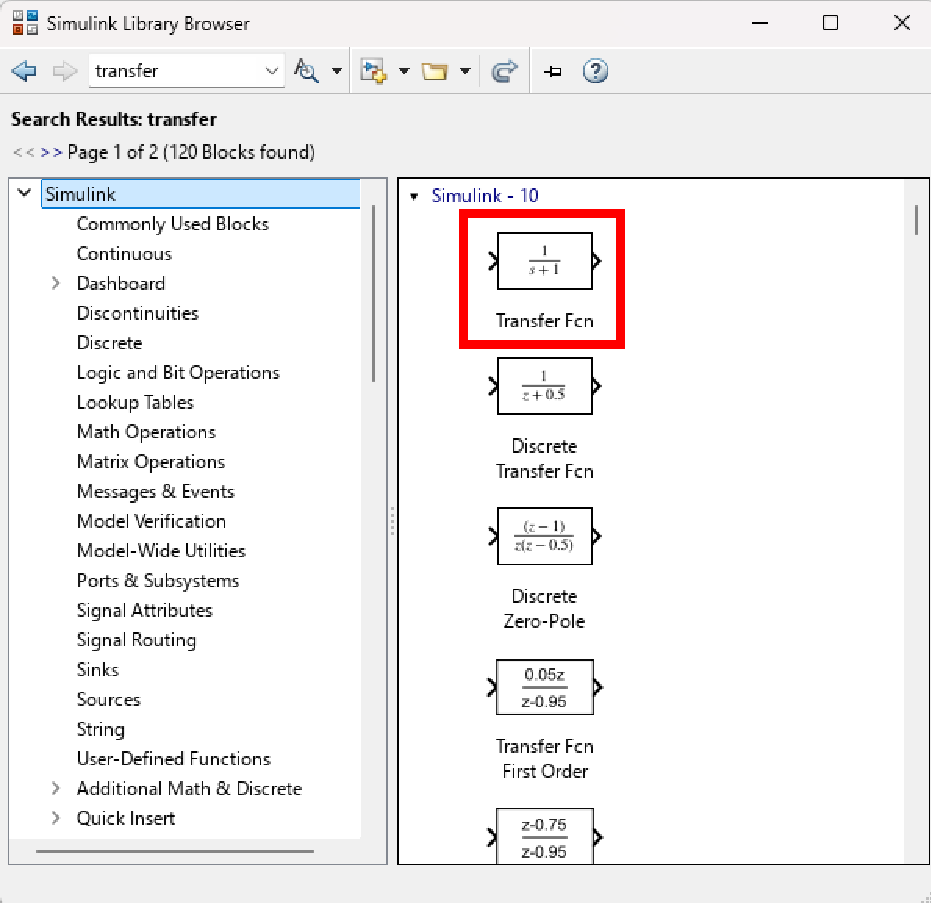
\includegraphics[width=\textwidth]{fig/Capitulo5/Caso_de_estudio_PID/Transfer_func.pdf}
        \caption{Librería de bloques - Funcion de trasnferencia}
        \label{fig:tf_func_lib}
    \end{subfigure}
    \hfill
    \begin{subfigure}[b]{0.45\textwidth}
        \centering
        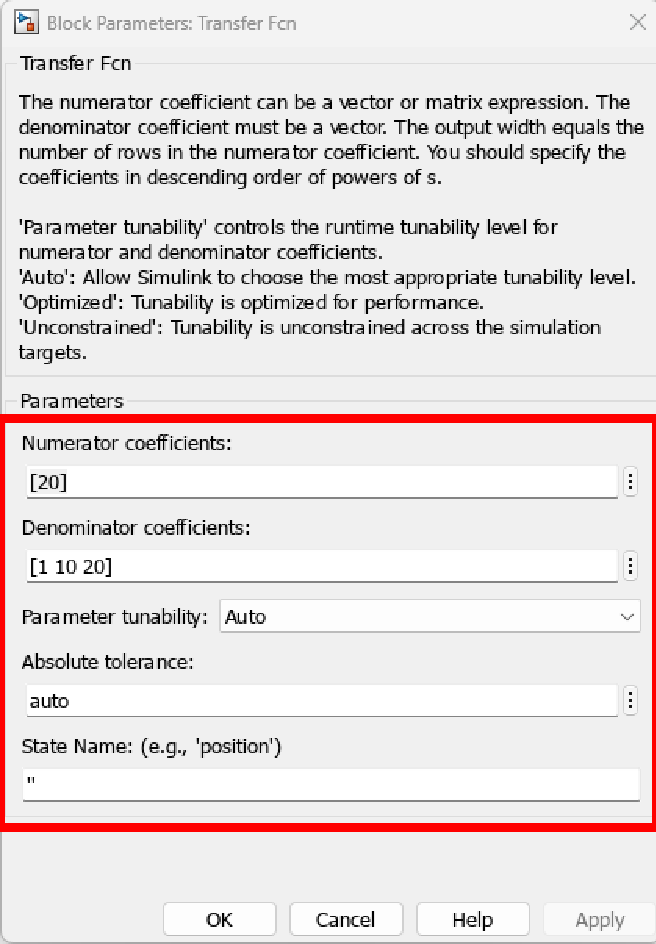
\includegraphics[width=\textwidth]{fig/Capitulo5/Caso_de_estudio_PID/config_transfer_function.pdf}
        \caption{Configuración del bloque encargado de aplicar la funcion de transferencia}
        \label{fig:tf_func_conf}
    \end{subfigure}
    \caption{Bloque funcion de transferencia}
    \label{fig:tf_func_block}
\end{figure}

Al tratase de la implementacion de un control PID el mismo debe de contar con la funcion de transferencia, esta se implementa mediante el bloque que se muestra en la Figura \ref{tf_func_block}, el mismo se encuentra en la libreria de bloques como se observa en la Figura \ref{fig:tf_func_lib}, ademas de esto la configuracion de la funcion de transferencia se puede observar en la Figura \ref{fig:tf_func_conf}.

%%gain
\begin{figure}[htbp]
    \centering
    % Primera imagen
    \begin{subfigure}[b]{0.35\textwidth}
        \centering
        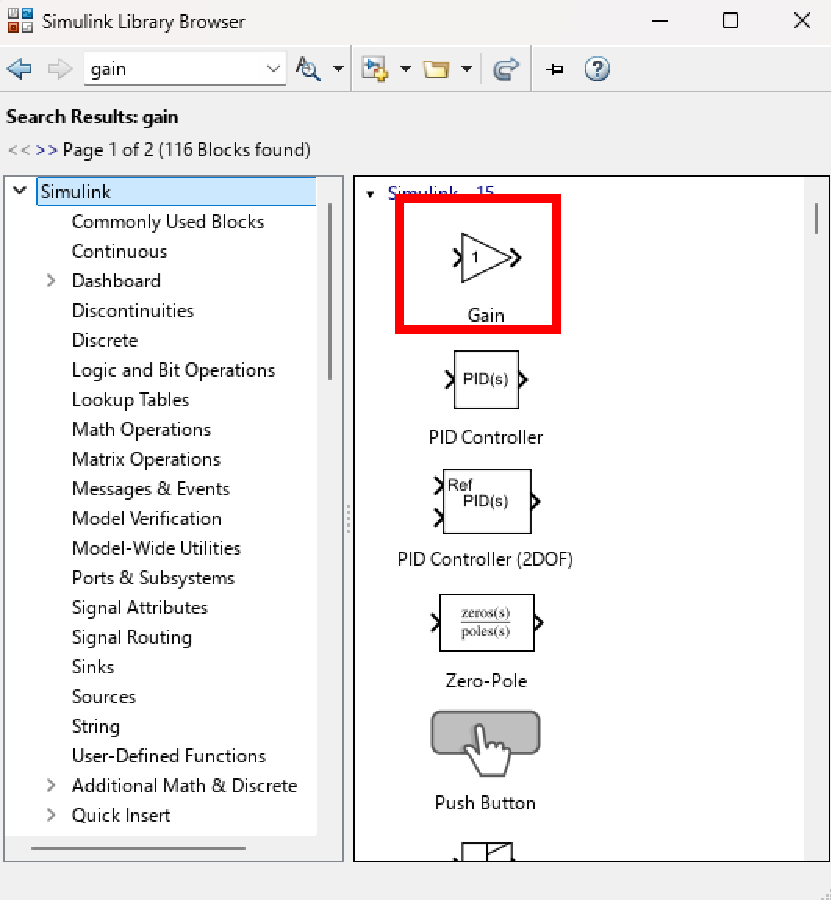
\includegraphics[width=\textwidth]{fig/Capitulo5/Caso_de_estudio_PID/lib_gain.pdf}
        \caption{Librería de bloques - Ganancia}
        \label{fig:lib_bloques_gain}
    \end{subfigure}
    \hfill
    % Segunda imagen
    \begin{subfigure}[b]{0.45\textwidth}
        \centering
        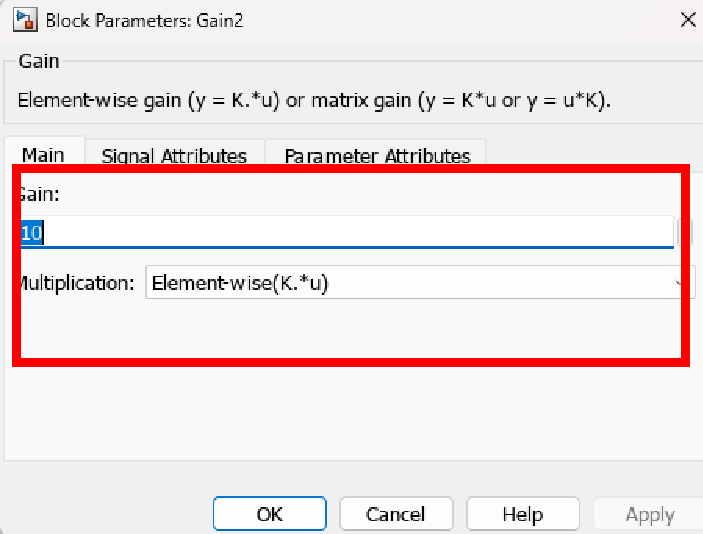
\includegraphics[width=\textwidth]{fig/Capitulo5/Caso_de_estudio_PID/config_gain_10.pdf}
        \caption{Configuración de parámetros 1}
        \label{fig:parametros_gain_01}
    \end{subfigure}
    \hfill
    % Tercera imagen
    \begin{subfigure}[b]{0.45\textwidth}
        \centering
        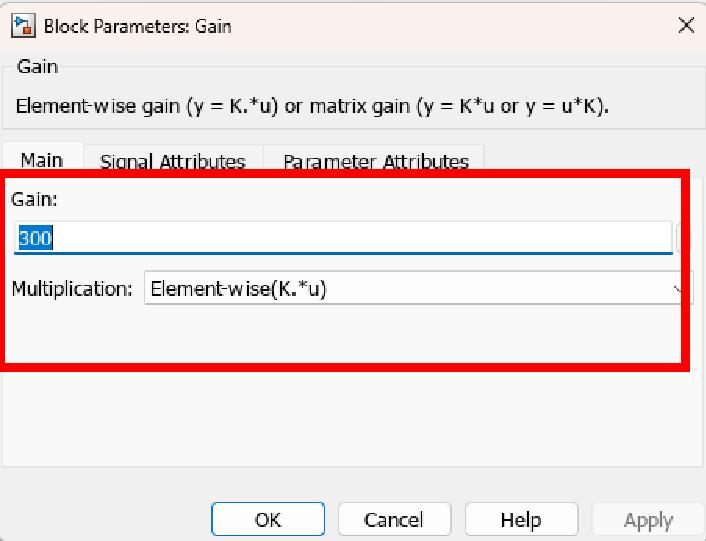
\includegraphics[width=\textwidth]{fig/Capitulo5/Caso_de_estudio_PID/config_gain_300.pdf}
        \caption{Configuración de parámetros 2}
        \label{fig:parametros_gain_02}
    \end{subfigure}
    \hfill
    % Cuarta imagen
    \begin{subfigure}[b]{0.45\textwidth}
        \centering
        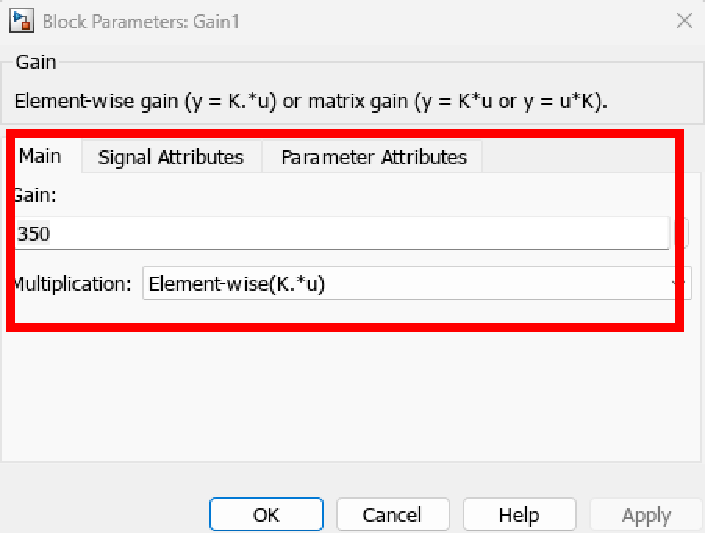
\includegraphics[width=\textwidth]{fig/Capitulo5/Caso_de_estudio_PID/config_gain_350.pdf}
        \caption{Configuración de parámetros 3}
        \label{fig:parametros_gain_03}
    \end{subfigure}

    \caption{Bloque para la asignación de ganancias}
    \label{fig:arreglo_gain}
\end{figure}

Tambien se deben de ingresar los valores de las ganancias esto se realiza por medio del bloque que se muestra en la Figura \ref{fig:arreglo_gain}, se logra mediante la implementacion de 3 bloques de ganancia el primero se genera con la configuracion que se muestra en la Figura \ref{fig:parametros_gain_01}, el segundo se establece segun los parametros indicados en la Figura \ref{fig:parametros_gain_02} y finalmente el tercero se establece como lo indica la Figura \ref{fig:parametros_gain_03}. 

%%add
\begin{figure}[htbp]
    \centering
    % Primera imagen
    \begin{subfigure}[b]{0.35\textwidth}
        \centering
        \includegraphics[width=\textwidth]{fig/Capitulo5/Caso_de_estudio_PID/lib_suma.pdf}
        \caption{Librería de bloques - suma}
        \label{fig:lib_bloques_add}
    \end{subfigure}
    \hfill
    % Segunda imagen
    \begin{subfigure}[b]{0.45\textwidth}
        \centering
        \includegraphics[width=\textwidth]{fig/Capitulo5/Caso_de_estudio_PID/config_sum_02.pdf}
        \caption{Configuración de parámetros 1}
        \label{fig:parametros_add_01}
    \end{subfigure}
    \hfill
    % Tercera imagen
    \begin{subfigure}[b]{0.45\textwidth}
        \centering
        \includegraphics[width=\textwidth]{fig/Capitulo5/Caso_de_estudio_PID/config_sum_01.pdf}
        \caption{Configuración de parámetros 2}
        \label{fig:parametros_add_02}
    \end{subfigure}

    \caption{Bloques encargados de sumas}
    \label{fig:arreglo_add}
\end{figure}

\newpage

Finalmente se deben de implementar dos bloques de suma, el primer bloque se encarga de realizar la realimentacion del sistema de control, el mismo se implementa haciendo uso de bloque de la libreria que se observa en la Figura \ref{fig:lib_bloques_add}, esto mediante el uso de la configuracion que se establece en la Figura \ref{fig:parametros_add_01}, por otro lado el segundo bloque de suma se encarga de sumar las tres senales de salida del controlador PID este bloque se debe de configurar como se muestra en la Figura \ref{fig:parametros_add_02}. Una vez implementado el sistema el archivo se debera de guardar bajo el nombre de (PIDRunFile) y el tiempo de ejecucio se debe de establecer en 0.5ms. 

\subsection{Resultados simulados}\label{subsub:resultados_simulados_PID}

\begin{figure}[h!]
    \centering
    \includegraphics[width=0.8\textwidth]{fig/Capitulo5/Caso_de_estudio_PID/datos/simulada.png}
    \caption{Salida simulada - PID }
    \label{fig:salida_simulada_PID}
\end{figure}


Ejecutando el sistema en el entorno de simulacion MATLAB Simulink se obtienen los resutlados que se muestran en \ref{fig:salida_simulada_PID}. Cabe estacar que el resultado es esperado, ya que el valor de estado estacionario esperado para este modelo debería ser de 1.02 V. En las próximas secciones se detallaran los pasos a seguir para la implementación de este sistema en la tarjeta de desarrollo por medio del flujo de trabajo desarrollado en en capítulo \ref{ch:especifico2}. 


\subsection{Implementación en la Tarjeta de desarrollo mediante EmbedSynthGNC}

Para la implementación en la tarjeta de desarrollo ZedBoard se ejecuta el flujo de trabajo que se muestra en la sección \ref{sec:m2m_transformator}. El mismo es representado mediante el diagrama que se muestra en la Figura \ref{fig:m2m_matlab_simulink_coder}.

Primeramente se deben de generar los archivos de Codigo C desde MATLAB Simulink, para esto se deben de seguir el diagrama de la Figura \ref{fig:m2m_matlab_simulink_coder}. 

\begin{figure}[h!]
    \centering
    \includegraphics[width=0.5\textwidth]{fig/especifico_2/CASO_ESTUDIO_FILTRO/Diagrama matlab simulink scope.pdf}
    \caption{Definición del procesador objetivo y arquitectura}
    \label{fig:system_target_PID}
\end{figure}

Seguido de esto como se muestra en la Figura \ref{fig:system_target_PID} se debe de establecer el procesador objetivo y la arquitectura del mismo.Finalmente se debe de definir el tipo de archivo de construccion el cual se puede observar en la Figura \ref{fig:pestana_config_output_file}. 

El archivo resultante sera un archivo llamado PIDRunFile.zip seguido de esto se debe de  se exportan los archivos al sistema Linux. Una vez exportados los archivos se descomprimen los mismos en la carpeta denominada swap area.

\begin{figure}[h!]
    \centering
    \includegraphics[width=0.5\textwidth]{fig/Capitulo5/Caso_de_estudio_PID/retornos_consola/Screenshot from 2024-10-31 20-21-37.png}
    \caption{Archivo de construcción en el directorio swap area}
    \label{fig:swap_area_PID}
\end{figure}


\begin{lstlisting}[language=bash, caption={Compilacion del programa , Linux}, label=lst:build_cmake_file_PID]
    cmake -DCMAKE_C_COMPILER=arm-linux-gnueabihf-gcc 
    CMakeLists.txt -DMATLAB_ROOT=/home/test/PIDRunFile/R2024b/
\end{lstlisting}

Una vez descomprimidos los archivos en el directorio denominado como swap area se deben enviar al contenedor mediante el comando que se muestra en \ref{fig:swap_area_PID}. Una vez dentro del contenedor se debe construir el archivo responsable de la compilacion del codigo C, esto se logra mediante el comando que se muestra en \ref{lst:build_cmake_file_PID}. El archivo binario resultante se encuentra en la ruta /home/PIDRunFile/casodeestudiopid, el mismo se debe de enviar al directorio denominado swap area, este se debe de exportar al contenedor encargado de integrarlo a la imagen generada mediante el marco de trabajo de Yocto y el flujo de trabajo de EmbedSynthGNC. 


Una vez dentro del contendor se debe de ir al directorio denominado meta-EmbedSynthGNC dentro del mismo se debe ingresar a la ruta /poky/meta-EmbedsinthGNC/recipes-core y en la misma se debe agregar un directorio con el nombre de (pid). Ademas de esto se debe inicializar el ambiente de trabajo mediante el uso del comando \ref{lst:yocto_ambient_set}. Una vez inicializado el ambiente de trabajo se debe agregar la nueva capa generada al archivo deniminado local.conf esto con el fin que el binario con el nombre PIDRunFile sea incluido en la generación de la imagen. Una vez generada la imagen se deben repetir los pasos que se muestran en \ref{sub:image2zedboard} donde se contempla exportar los archivos contenidos en la ruta xxxxx. Seguido de esto se debe preparar la memoria extraible de la tarjeta de desarrollo para los nuevos archivos.


\subsection{Resultados de la implementación}

\begin{figure}[htbp]
    \centering
    \begin{subfigure}[b]{0.35\textwidth}
        \centering
        \includegraphics[width=\textwidth]{fig/Capitulo5/Caso_de_estudio_IMU/Generador_de_salidas/libreria_bloque_de_funcion.pdf}
        \caption{Tarjeta de desarrollo ZedBoard - PID}
        \label{fig:PID_zedboard}
    \end{subfigure}
    \hfill
    \begin{subfigure}[b]{0.45\textwidth}
        \centering
        \includegraphics[width=\textwidth]{fig/Capitulo5/Caso_de_estudio_IMU/Generador_de_salidas/configuracion_codigo.pdf}
        \caption{Archivos de salida}
        \label{fig:out_files_PID}
    \end{subfigure}
    \caption{Programa PIDRunFile implementado en la tarjeta de desarrollo}
    \label{fig:PID_ZEDBOARD}
\end{figure}


Como se puede observar en la Figura \ref{fig:PID_zedboard} se observa el binario contenido en la imagen dentro de la tarjeta de desarrollo. Una vez ejecutado el mismo se obtienen los archivos de salida que se muestran en la Figura \ref{fig:out_files_PID}. 

\begin{figure}[h!]
    \centering
    \includegraphics[width=0.5\textwidth]{fig/Capitulo5/Caso_de_estudio_PID/datos/experimental.png}
    \caption{Gráfico de archivo de salida experimental}
    \label{fig:experimentales_PID}
\end{figure}

Analizando los mismos mediante el programa de Python \ref{apx:comparacion_de_sennales_programa} se obtienen los graficos que se muestran en \ref{fig:experimentales_PID}, en donde se muestra el grafico de xxxxx. Realizando la comparacion con los datos simulados obtenidos en \ref{subsub:resultados_simulados_PID}, se obtienen los siguientes resultados para el analisis de error.

\begin{itemize}
    \item Error Promedio Absoluto = $1.12\times 10^{-32}$ []
    \item Error Cuadrático Medio = $1.01 \times 10^{-34}$ $[^{2}]$
    \item Raíz del Error Cuadrático Medio = $1.01 \times 10{-17}$ []
\end{itemize}


Los resultados obtenidos en el análisis de error muestran valores extremadamente bajos, indicando una alta concordancia entre las señales comparadas. El Error Promedio Absoluto de $1.12\times 10^{-32}$ sugiere que las desviaciones promedio entre los datos experimentales y simulados son insignificantes, mientras que el Error Cuadrático Medio de 
 $1.01 \times 10^{-34}$  refuerza este resultado al reflejar un bajo nivel de variabilidad en los errores al cuadrado. Finalmente, la Raíz del Error Cuadrático Medio (RMSE), con un valor de $1.01 \times 10{-17}$ , confirma que las diferencias entre las señales son prácticamente despreciables, lo cual respalda la precisión del modelo simulado respecto al proceso experimental. Estos valores en conjunto demuestran una correspondencia casi exacta, validando la efectividad del modelo para replicar el comportamiento de la señal experimental.

\section{Reflexión final}


La implementación y análisis de dos casos de estudio, uno centrado en el uso de una Unidad de Medición Inercial (IMU) y otro en un controlador PID, han revelado resultados con errores notablemente bajos, lo que indica una alta precisión en ambos enfoques. La IMU, con su capacidad para medir aceleración y velocidad angular en tiempo real, mostró una correspondencia significativa entre los datos experimentales y los simulados. Los valores de error, casi nulos, sugieren que el modelo simulado captura con gran exactitud las dinámicas y variaciones de los movimientos medidos, lo cual es esencial para aplicaciones que requieren un monitoreo preciso de la orientación y posición en entornos críticos. La efectividad del modelo IMU indica que se puede confiar en los datos simulados como una representación fiel del comportamiento del sistema en condiciones reales.

De manera similar, el controlador PID logró un ajuste excepcionalmente alto entre la señal deseada y la respuesta obtenida en la simulación, con errores prácticamente despreciables que demuestran un control preciso sobre la señal en cuestión. La baja magnitud de error en ambos casos sugiere que el sistema de control es altamente efectivo en términos de corrección de desviaciones y en la capacidad del modelo para minimizar las diferencias entre los datos simulados y experimentales. Estos resultados no solo validan el rigor de las simulaciones y la calidad del modelado, sino que también brindan una base sólida para futuras aplicaciones y ajustes, dado que los modelos son capaces de replicar de manera precisa el comportamiento de sistemas reales. La consistencia en los bajos valores de error en ambos casos de estudio subraya la confiabilidad y aplicabilidad de estos modelos en escenarios de guía, navegación y control, donde la precisión es fundamental.